% !TEX encoding = UTF-8 Unicode 
%
% Use:
% magister / inzynier - for master thesis or engineering thesis
% druk / archiwum - for print version or archive version
% en - to translate template into english
% examples:
%\documentclass[inzynier,druk,en] - master thesis, print version, english
%\documentclass[magister,druk,en]{dyplom}
%\documentclass[magister,druk]{dyplom}

\documentclass[magister,druk]{dyplom}

\usepackage[utf8]{inputenc}
\usepackage{hyperref}

% Maximum section's depth.
\setcounter{secnumdepth}{4}

% Listings settings
\setminted{breaklines, 
frame=lines,           
framesep=3mm,          
baselinestretch=1.1,   
fontsize=\small,       
% linenos              % line numbering
}

\usepackage{lipsum}

% \faculty{Faculty of \dots}                   % Uncomment if applicable
\fieldofstudy{Zaufane Systemy Sztucznej Inteligencji}                          
\author{Paweł Pelar}
\title{Badanie wpływu tła na klasyfikację zwierząt na obrazach}
\supervisor{dr hab. inż. Henryk Maciejewski}
% \consultant{Consultant's name}               % Uncomment if applicable
% \specialisation{AAA}                         % Uncomment if applicable
\keywords{classification, image segmentation}	% 3-5 keywords  

\begin{document}

\maketitle

\abstract{
% English abstract 

\lipsum[1]

}{
% Abstract translated into Polish

\lipsum[2]

}

\tableofcontents

% !TEX encoding = UTF-8 Unicode 
% !TEX root = praca.tex

\chapter*{Wprowadznie}

W ostatnich latach technologia głębokiego uczenia maszynowego zrewolucjonizowała dziedzinę
przetwarzania obrazów, w tym klasyfikację i segmentację obrazów. Klasyfikacja obrazów, 
czyli proces przypisywania etykiet do obiektów przedstawionych na obrazach, jest fundamentalnym
zagadnieniem w komputerowym rozpoznawaniu wzorców. Pomimo znaczących postępów, istnieje wiele 
czynników, które mogą wpływać na dokładność i niezawodność modeli klasyfikacyjnych, a jednym z 
kluczowych elementów jest tło obrazu.

Tło obrazu może dostarczać zbędnych informacji lub wprowadzać modele w błąd, co może prowadzić 
do błędnej klasyfikacji obiektów. W szczególności w kontekście klasyfikacji zwierząt, obecność 
złożonego lub niestandardowego tła może znacząco wpłynąć na wyniki klasyfikacji. Dlatego analiza 
wpływu tła na wyniki klasyfikacji obrazów jest niezwykle istotna dla poprawy efektywności modeli.

Segmentacja obrazów, czyli proces podziału obrazu na mniejsze, znaczące fragmenty, jest jednym z 
podejść umożliwiających radzenie sobie z problemem tła. Dzięki segmentacji możliwe jest wydzielenie 
obiektu z tła, co może prowadzić do poprawy wyników klasyfikacji. W niniejszej pracy zostaną 
wykorzystane gotowe modele do segmentacji obrazów, w celu usunięcia tła, w celu przeprowadzenia 
późniejszych modyfikacji tła.

Wyzwania związane z klasyfikacją obrazów i segmentacją obejmują m.in. różnorodność danych, 
obecność zakłócających elementów w tle, zmienność oświetlenia oraz różnice w skalach obiektów. 
Zastosowanie zaawansowanych technik segmentacji i analizy wpływu tła może jednak znacząco poprawić
wyniki klasyfikacji.

Niniejsza praca wnosi istotny wkład do dziedziny przetwarzania obrazów, oferując nowe spostrzeżenia
na temat wpływu tła na klasyfikację oraz oceniając skuteczność różnych modeli głębokiego uczenia w 
kontekście zmiennych warunków tła. Przeprowadzone badania mają na celu pogłębienie wiedzy na temat 
optymalizacji modeli klasyfikacyjnych w złożonych i zmiennych środowiskach.

\section*{Cel pracy}

Celem niniejszej pracy jest zbadanie wpływu tła na klasyfikację zwierząt na obrazach przy 
użyciu zaawansowanych modeli głębokiego uczenia, takich jak ResNet i ConvNeXt. Kluczowym aspektem 
tego badania jest ocena, w jaki sposób usunięcie i modyfikacja tła wpływają na wydajność tych modeli 
klasyfikacyjnych. Poprzez analizę wyników przed i po modyfikacji tła, praca ta ma na celu:

\begin{itemize}
    \item \textbf{Ocena wrażliwości modeli na tło:} Sprawdzenie, jak różne rodzaje tła wpływają na 
    dokładność klasyfikacji obrazów zwierząt. Analiza ta pozwoli zrozumieć, w jakim stopniu obecność 
    tła zakłóca proces klasyfikacji i jakie rodzaje czy modyfikacje tła mają największy wpływ na wyniki.
    \item \textbf{Optymalizacja procesu klasyfikacji:} Zidentyfikowanie najlepszych praktyk i metod 
    usuwania oraz modyfikacji tła, które mogą poprawić wydajność modeli klasyfikacyjnych. Badanie to 
    pozwoli określić, które techniki segmentacji i modyfikacji tła są najbardziej efektywne w 
    kontekście różnych modeli klasyfikacyjnych.
    \item \textbf{Porównanie wydajności modeli:} Porównanie jakości klasyfikacji przy użyciu różnych 
    modeli głębokiego uczenia w kontekście zmiennych warunków tła. Analiza ta pozwoli zidentyfikować, 
    który model lepiej radzi sobie z problemem tła i jest bardziej odporny na jego zmiany.
    \item \textbf{Praktyczne implikacje:} Dostarczenie praktycznych wskazówek i rekomendacji 
    dotyczących zastosowania modeli głębokiego uczenia w zadaniach klasyfikacji obrazów w warunkach 
    rzeczywistych, gdzie tło może być zmienne i nieprzewidywalne. Wnioski z tego badania mogą być 
    użyteczne dla badaczy i praktyków zajmujących się rozpoznawaniem obrazów w różnych dziedzinach, 
    takich jak ekologia, bezpieczeństwo czy medycyna.
\end{itemize}

\section*{Zakres pracy}

Zakres pracy obejmuję kilka kluczowych aspektów, a mianowicie:

\begin{enumerate}
    \item \textbf{Przygotowanie środowiska badawczego:}
    \begin{itemize}
        \item Konfiguracja niezbędnego oprogramowania i bibliotek do przetwarzania obrazów 
        oraz uczenia maszynowego.
        \item Ustalenie parametrów eksperymentalnych i kryteriów oceny.
    \end{itemize}
    \item \textbf{Przygotowanie danych:}
    \begin{itemize}
        \item Zebranie odpowiednich zbiorów danych zawierających obrazy zwierząt z różnorodnym tłem.
        \item Przeprowadzenie potrzebnego preprocessingu danych.
    \end{itemize}
    \item \textbf{Wykorzystanie gotowych modeli klasyfikacyjnych:}
    \begin{itemize}
        \item Wykorzystanie istniejących, wytrenowanych modeli do klasyfikacji obrazów.
        \item Przeprowadzenie wstępnych ocen wydajności modeli na oryginalnych obrazach z różnym tłem.
    \end{itemize}
    \item \textbf{Segmentacja obrazów:}
    \begin{itemize}
        \item Wykorzystanie gotowego modelu segmentacyjnego do usunięcia tła z obrazów.
        \item Walidacja i ocena uzyskanych masek i obrazów.
    \end{itemize}
    \item \textbf{Modyfikacja tła obrazów:}
    \begin{itemize}
        \item Zastosowanie różnych technik modyfikacji tła w celu stworzenia zestawów danych z różnymi 
        wariantami tła.
        \item Analiza wpływu tych modyfikacji na jakość klasyfikacji.
    \end{itemize}
    \item \textbf{Ocena i analiza wyników:}
    \begin{itemize}
        \item Porównanie wyników klasyfikacji przed i po modyfikacjach tła za pomocą wybranych metryk.
        \item Interpretacja wyników oraz wyciągnięcie wniosków dotyczących wpływu tła na wydajność modeli 
        klasyfikacyjnych.
    \end{itemize}
    \item \textbf{Wnioski i rekomendacje:}
    \begin{itemize}
        \item Sformułowanie wniosków na podstawie przeprowadzonych eksperymentów.
        \item Propozycja potencjalnych kierunków dalszych badań oraz zastosowań praktycznych.
    \end{itemize}
\end{enumerate}

\chapter*{Przegląd literatury}

W ramach niniejszego rozdziału przedstawiony zostanie przegląd literatury dotyczący 
kluczowych zagadnień związanych z klasyfikacją obrazów, segmentacją obrazów oraz wpływem 
tła na wyniki klasyfikacji. Celem tego przeglądu jest zrozumienie dotychczasowych badań i rozwiązań, 
które mogą być istotne dla realizacji niniejszej pracy. Omówione zostaną zarówno klasyczne, jak i 
nowoczesne podejścia do tych problemów, ze szczególnym uwzględnieniem zaawansowanych modeli głębokiego 
uczenia, takich jak ResNet i ConvNeXt. Przegląd ten pozwoli na identyfikację luk w istniejącej 
literaturze oraz wskazanie potencjalnych kierunków dalszych badań.

\section*{Zakres przeglądu literatury}

\begin{enumerate}
    \item \textbf{Klasyfikacja obrazów:}
    \begin{itemize}
        \item Historia i ewolucja metod klasyfikacji obrazów.
        \item Przegląd tradycyjnych technik, takich jak SVM i K-NN, oraz ich ograniczeń.
        \item Wprowadzenie do modeli głębokiego uczenia, w tym sieci neuronowych i 
        konwolucyjnych sieci neuronowych (CNN).
    \end{itemize}
    \item \textbf{Modele głębokiego uczenia:}
    \begin{itemize}
        \item Szczegółowy przegląd architektur ResNet i ConvNeXt.
        \item Analiza wyników i wydajności tych modeli w różnych zadaniach klasyfikacji.
        \item Porównanie ResNet i ConvNeXt z innymi popularnymi modelami, takimi jak VGG i Inception.
    \end{itemize}
    \item \textbf{Segmentacja obrazów:}
    \begin{itemize}
        \item Przegląd technik segmentacji obrazów, w tym tradycyjnych metod oraz 
        podejść opartych na głębokim uczeniu.
        \item Modele segmentacyjne takie jak U-Net, Mask R-CNN i inne.
        \item Zastosowania segmentacji obrazów w różnych dziedzinach.
    \end{itemize}
    \item \textbf{Wpływ tła na klasyfikację obrazów:}
    \begin{itemize}
        \item Przegląd badań dotyczących wpływu tła na wyniki klasyfikacji obrazów.
        \item Techniki usuwania i modyfikacji tła oraz ich efektywność.
        \item Przykłady zastosowań w praktyce i analiza wyników.
    \end{itemize}
    \item \textbf{Metryki oceny jakości modeli:}
    \begin{itemize}
        \item Omówienie metryk używanych do oceny jakości modeli klasyfikacyjnych i segmentacyjnych.
        \item Dokładność, precyzja, recall, F1-score i inne miary.
    \end{itemize}
\end{enumerate}

\section*{Cel przeglądu literatury}
Celem przeglądu literatury jest dostarczenie kompleksowej wiedzy na temat aktualnego stanu badań
i technologii w obszarze klasyfikacji i segmentacji obrazów. Przegląd ten pozwoli na:

\begin{itemize}
    \item Zidentyfikowanie najnowszych osiągnięć i trendów w dziedzinie przetwarzania obrazów.
    \item Zrozumienie, jakie techniki i modele są obecnie uważane za najbardziej efektywne.
    \item Wskazanie luk w istniejących badaniach, które mogą stanowić podstawę do dalszych badań.
    \item Sformułowanie wniosków i rekomendacji na temat optymalnych podejść do rozwiązania problemu wpływu tła na klasyfikację obrazów.
\end{itemize}

\section*{Klasyfikacja obrazów}

Klasyfikacja obrazów to jedno z fundamentalnych zadań w dziedzinie przetwarzania obrazów i 
komputerowego rozpoznawania wzorców. Proces ten polega na przypisaniu każdemu obrazowi jednej 
lub więcej etykiet z predefiniowanego zbioru klas. Technologia ta znalazła zastosowanie w wielu 
dziedzinach, takich jak medycyna, bezpieczeństwo, rolnictwo, czy automatyka przemysłowa. W ramach 
tego przeglądu omówione zostaną tradycyjne metody klasyfikacji obrazów, ewolucja podejść z 
wykorzystaniem głębokiego uczenia oraz zaawansowane architektury sieci neuronowych.

\subsection*{Tradycyjne metody klasyfikacji obrazów}

W początkowych etapach rozwoju klasyfikacji obrazów stosowano głównie techniki oparte
na ręcznie wyodrębnianych cechach oraz klasyfikatorach statystycznych. Do najbardziej
popularnych metod należały:

\begin{itemize}
    \item \textbf{Support Vector Machines (SVM):} Technika ta polega na znajdowaniu hiperpowierzchni, 
    która najlepiej rozdziela klasy w przestrzeni cech. SVM były szeroko stosowane w klasyfikacji 
    obrazów dzięki swojej skuteczności w radzeniu sobie z nieliniowymi danymi poprzez zastosowanie 
    funkcji jądrowych.
    \item \textbf{K-Nearest Neighbors (K-NN):} Algorytm ten klasyfikuje nowy przykład na podstawie 
    większości głosów najbliższych sąsiadów w przestrzeni cech. Pomimo swojej prostoty, K-NN często 
    wymaga dużych zasobów obliczeniowych i pamięciowych, szczególnie przy dużych zbiorach danych.
    \item \textbf{Metody oparte na histogramach cech:} Techniki takie jak Histogram of Oriented 
    Gradients (HOG) czy Scale-Invariant Feature Transform (SIFT) były używane do ekstrakcji cech z 
    obrazów, które następnie były klasyfikowane za pomocą modeli takich jak SVM czy K-NN.
\end{itemize}

\subsection*{Ewolucja podejść z wykorzystaniem głębokiego uczenia}

Wraz z rozwojem technologii głębokiego uczenia, tradycyjne metody zaczęły ustępować 
miejsca konwolucyjnym sieciom neuronowym (CNN), które zrewolucjonizowały klasyfikację obrazów. 
CNN automatycznie uczą się cech bez potrzeby ręcznego ich wyodrębniania, co pozwala na osiąganie 
znacznie lepszych wyników.

\begin{itemize}
    \item \textbf{Convolutional Neural Networks (CNN):} CNN składają się z warstw konwolucyjnych, 
    poolingowych i w pełni połączonych, które są trenowane w sposób end-to-end na surowych danych 
    obrazowych. Pionierskie prace takie jak AlexNet, VGG i GoogLeNet zapoczątkowały erę głębokiego 
    uczenia w klasyfikacji obrazów, osiągając znacznie lepsze wyniki niż tradycyjne metody.
    \item \textbf{Residual Networks (ResNet):}  Wprowadzenie ResNet w 2015 roku było przełomem 
    w dziedzinie głębokiego uczenia. ResNet wprowadza pojęcie "residual learning" z wykorzystaniem 
    warstw skrótowych (skip connections), co pozwala na trenowanie bardzo głębokich sieci z tysiącami 
    warstw bez problemu zanikania gradientu.
    \item \textbf{Transformers} Chociaż pierwotnie zaprojektowane do przetwarzania języka naturalnego, 
    architektury oparte na transformerach, takie jak Vision Transformer (ViT), zaczęły być stosowane 
    również w klasyfikacji obrazów. Transformery wykorzystują mechanizm uwagi (attention mechanism), 
    co pozwala na modelowanie globalnych zależności w danych.
\end{itemize}

\subsection*{Zaawansowane architektury sieci neuronowych}

Obecnie w klasyfikacji obrazów stosuje się wiele zaawansowanych architektur, 
które rozwijają i ulepszają wcześniejsze koncepcje:

\begin{itemize}
    \item \textbf{ConvNeXt:} Jest to nowoczesna architektura CNN, która łączy zalety tradycyjnych 
    konwolucyjnych sieci neuronowych z nowymi pomysłami pochodzącymi od transformerów. 
    ConvNeXt wykorzystuje bardziej złożone operacje konwolucyjne oraz zaawansowane techniki 
    normalizacji, co pozwala na osiąganie znakomitych wyników w różnych zadaniach klasyfikacji.
    \item \textbf{EfficientNet:}  EfficientNet wprowadza skalowanie sieci, które jednocześnie 
    zwiększa głębokość, szerokość i rozdzielczość sieci w zrównoważony sposób. Podejście to 
    pozwala na tworzenie modeli, które są bardziej efektywne obliczeniowo i mogą osiągać wyższą 
    dokładność przy mniejszym zużyciu zasobów.
\end{itemize}

\subsection*{Podsumowanie}
Przegląd literatury dotyczącej klasyfikacji obrazów pokazuje, jak ewoluowały metody od 
tradycyjnych technik opartych na ręcznie wyodrębnianych cechach do zaawansowanych modeli 
głębokiego uczenia. Nowoczesne architektury, takie jak ResNet i ConvNeXt, oferują znakomite 
wyniki i są obecnie standardem w wielu zastosowaniach przemysłowych i naukowych. Zrozumienie 
tych technologii i ich rozwoju jest kluczowe dla dalszych badań i optymalizacji modeli 
klasyfikacyjnych, zwłaszcza w kontekście analizy wpływu tła na wyniki klasyfikacji obrazów.

\section*{Modele głębokiego uczenia}

Modele głębokiego uczenia, zwłaszcza konwolucyjne sieci neuronowe (CNN), zrewolucjonizowały 
przetwarzanie obrazów, w tym zadania takie jak klasyfikacja, detekcja obiektów, i segmentacja. 
W ramach tego przeglądu literatury skupimy się na najbardziej wpływowych modelach głębokiego uczenia, 
w tym na ich architekturach, kluczowych innowacjach oraz wynikach osiągniętych na różnych benchmarkach.

\subsection*{Convolutional Neural Networks (CNN)}

CNN są fundamentem nowoczesnego przetwarzania obrazów. Ich struktura składa się z warstw 
konwolucyjnych, poolingowych i w pełni połączonych, które są trenowane w sposób end-to-end. 
AlexNet, zaprojektowany przez Krizhevsky'ego, Sutskevera i Hinton’a w 2012 roku, był pierwszym 
modelem, który pokazał ogromny potencjał głębokiego uczenia w zadaniach klasyfikacji obrazów. 
Wprowadzenie dużych filtrów konwolucyjnych, warstw max-pooling oraz technik regularizacji takich 
jak dropout przyczyniło się do znacznego zmniejszenia błędu klasyfikacji na konkursie ImageNet. 
Kolejnym krokiem w rozwoju CNN było VGGNet, opracowane przez Simonyana i Zissermana w 2014 roku. 
VGGNet zyskało popularność dzięki swojej prostocie i skuteczności, opierając się na małych filtrach 
konwolucyjnych (3x3) oraz głębokiej architekturze składającej się z wielu warstw konwolucyjnych. 
Model ten udowodnił, że zwiększenie głębokości sieci może prowadzić do lepszej wydajności.

GoogLeNet, zaprezentowany przez zespół Google w 2014 roku, wprowadził koncepcję "Inception modules", 
które umożliwiają efektywne równoległe przetwarzanie danych. Inception modules łączą różne wielkości 
filtrów konwolucyjnych w jednej warstwie, co pozwala na lepsze uchwycenie różnorodnych cech obrazu. 
Dodatkowo, zamiast tradycyjnych w pełni połączonych warstw na końcu sieci, GoogLeNet używa warstw 
global average pooling, co zmniejsza liczbę parametrów i zwiększa efektywność modelu. 
Model ten osiągnął świetne wyniki na ImageNet, redukując liczbę parametrów w porównaniu do 
wcześniejszych architektur.

\subsection*{Residual Networks (ResNet)}

W 2015 roku He et al. wprowadzili Residual Networks (ResNet), które zrewolucjonizowały głębokie 
uczenie. Kluczową innowacją w ResNet było wprowadzenie warstw skrótowych (skip connections), które 
umożliwiają trenowanie bardzo głębokich sieci poprzez rozwiązanie problemu zanikania gradientu. 
Dzięki temu podejściu możliwe stało się trenowanie sieci o głębokości nawet 152 warstw. ResNet 
osiągnął rewolucyjne wyniki na konkursie ImageNet, pokazując, że głębsze sieci mogą prowadzić do 
znacznie lepszej wydajności niż wcześniejsze architektury.

\subsection*{Transformery w przetwarzaniu obrazów}

Chociaż początkowo zaprojektowane do przetwarzania języka naturalnego, architektury oparte na 
transformerach znalazły zastosowanie również w przetwarzaniu obrazów. Vision Transformer (ViT), 
zaprezentowany przez Dosovitskiy'ego et al. w 2020 roku, adaptuje mechanizm uwagi 
(attention mechanism) do zadań przetwarzania obrazów. ViT dzieli obraz na mniejsze pliki 
(patches) i traktuje je jako tokeny w modelu transformera, co pozwala na globalne modelowanie 
zależności w danych. Model ten osiągnął konkurencyjne wyniki na benchmarkach takich jak ImageNet, 
udowadniając, że podejście oparte na transformerach może być równie skuteczne jak tradycyjne CNN.

\subsection*{Nowoczesne architektury}

Wśród nowoczesnych architektur CNN, ConvNeXt wyróżnia się jako model łączący zalety tradycyjnych 
konwolucyjnych sieci neuronowych z nowymi pomysłami pochodzącymi od transformerów. ConvNeXt 
wykorzystuje bardziej złożone operacje konwolucyjne oraz zaawansowane techniki normalizacji, 
co pozwala na osiąganie znakomitych wyników w różnych zadaniach klasyfikacji. Model ten potwierdza, 
że nowoczesne CNN mogą konkurować z modelami opartymi na transformerach.

EfficientNet, opracowany przez Tan i Le, wprowadza koncepcję skalowania sieci, która pozwala na 
jednoczesne zwiększanie głębokości, szerokości i rozdzielczości sieci w zrównoważony sposób. 
Dzięki podejściu zrównoważonego skalowania (compound scaling), EfficientNet tworzy modele, 
które są bardziej efektywne obliczeniowo i mogą osiągać wyższą dokładność przy mniejszym zużyciu 
zasobów. Model ten jest jednym z najbardziej efektywnych modeli głębokiego uczenia, osiągając 
wyższą dokładność przy optymalnym wykorzystaniu zasobów.

\subsection*{Podsumowanie}

Przegląd literatury dotyczącej modeli głębokiego uczenia w przetwarzaniu obrazów ukazuje dynamiczny 
rozwój tej dziedziny. Od wczesnych architektur CNN, takich jak AlexNet i VGG, przez innowacyjne 
podejścia ResNet i GoogLeNet, aż po nowoczesne modele ConvNeXt i transformery, takie jak ViT, 
ewolucja tych technologii znacząco poprawiła wyniki klasyfikacji obrazów. Zrozumienie tych 
innowacji i ich zastosowań jest kluczowe dla dalszych badań i optymalizacji modeli klasyfikacyjnych 
w różnych kontekstach, w tym w analizie wpływu tła na wyniki klasyfikacji obrazów.

\section*{Segmentacja obrazów}

Segmentacja obrazów to kluczowy proces w dziedzinie przetwarzania obrazów,
polegający na podziale obrazu na znaczące fragmenty, które mogą reprezentować 
różne obiekty lub regiony. Techniki segmentacji są szeroko stosowane w wielu dziedzinach,
takich jak medycyna, robotyka, analiza wideo i rozpoznawanie obiektów. W ramach tego przeglądu 
literatury omówione zostaną tradycyjne metody segmentacji, nowoczesne podejścia wykorzystujące 
głębokie uczenie oraz ich zastosowania w różnych kontekstach.

\subsection*{Tradycyjne metody segmentacji obrazów}

W początkowych etapach rozwoju segmentacji obrazów stosowano głównie metody oparte na analizie 
cech niskiego poziomu, takich jak kolor, tekstura i krawędzie. Do najpopularniejszych technik należały:

\begin{enumerate}
    \item \textbf{Segmentacja oparta na progach:} Technika ta polega na podziale obrazu na regiony 
    na podstawie wartości pikseli. Progi mogą być ustalane globalnie dla całego obrazu lub lokalnie 
    dla poszczególnych regionów. Chociaż metoda ta jest prosta, jej skuteczność zależy od 
    odpowiedniego doboru progów i jest ograniczona w przypadkach obrazów z złożonymi teksturami i 
    oświetleniem.
    \item \textbf{Segmentacja przez regiony:} Techniki takie jak algorytm wododziałowy (watershed 
    algorithm) oraz metoda region growing polegają na grupowaniu sąsiadujących pikseli o podobnych 
    wartościach. Algorytm wododziałowy modeluje obraz jako topograficzną mapę, gdzie linie 
    wododziałowe oddzielają różne segmenty. Metoda region growing natomiast zaczyna od zestawu 
    początkowych pikseli (seed points) i iteracyjnie dodaje sąsiednie piksele spełniające kryterium 
    podobieństwa.
    \item \textbf{Segmentacja oparta na krawędziach:} Metody te wykorzystują detekcję krawędzi 
    do identyfikacji granic między różnymi obiektami w obrazie. Algorytmy takie jak Canny edge 
    detector i Sobel operator są powszechnie stosowane do wykrywania krawędzi, które następnie 
    służą do segmentacji obrazu.
\end{enumerate}

\subsection*{Nowoczesne podejścia wykorzystujące głębokie uczenie}

Rozwój głębokiego uczenia wprowadził znaczące innowacje w dziedzinie segmentacji obrazów, 
zwłaszcza dzięki zastosowaniu konwolucyjnych sieci neuronowych (CNN). Modele te automatycznie 
uczą się reprezentacji cech z obrazów, co prowadzi do znacznie lepszej dokładności segmentacji w 
porównaniu do tradycyjnych metod.

\begin{enumerate}
    \item \textbf{Fully Convolutional Networks (FCN):} Wprowadzone przez Longa et al. w 2015 roku, 
    FCN przekształcają tradycyjne CNN, zastępując w pełni połączone warstwy konwolucyjnymi, co 
    pozwala na generowanie map segmentacji o tej samej rozdzielczości co wejściowy obraz. 
    FCN były pierwszym krokiem w kierunku end-to-end segmentacji obrazów.
    \item \textbf{U-Net:} Zaproponowany przez Ronnebergera et al. w 2015 roku, U-Net stał się 
    standardem w dziedzinie segmentacji medycznych obrazów. Architektura U-Net składa się z 
    symetrycznej struktury, która łączy warstwy składające się z konwolucji i upsamplingu, co 
    umożliwia precyzyjne segmentowanie obiektów. U-Net wyróżnia się również dzięki połączeniom 
    między warstwami, które przekazują szczegółowe informacje z warstw niskiego poziomu do warstw 
    wyższego poziomu, poprawiając dokładność segmentacji.
    \item \textbf{Mask R-CNN:} Rozwinięcie Faster R-CNN, Mask R-CNN, zaproponowane przez He et al. 
    w 2017 roku, rozszerza funkcjonalność detekcji obiektów o możliwość segmentacji. 
    Model ten dodaje gałąź segmentacyjną do istniejącej architektury detekcji obiektów, 
    umożliwiając precyzyjne maskowanie wykrytych obiektów. Mask R-CNN osiągnął znakomite 
    wyniki w wielu zadaniach segmentacji i detekcji obiektów.
    \item \textbf{DeepLab:} Rodzina modeli DeepLab, opracowana przez zespół Google, wykorzystuje 
    różne techniki do poprawy segmentacji, takie jak atrous convolutions (dylatowane konwolucje) i 
    Conditional Random Fields (CRFs). DeepLabv3+, najnowsza wersja tej serii, łączy atrous 
    convolutions z modulem spatial pyramid pooling, co pozwala na uchwycenie kontekstowych 
    informacji na różnych skalach.
\end{enumerate}

\subsection*{Zastosowania segmentacji obrazów}

Techniki segmentacji obrazów znalazły szerokie zastosowanie w różnych dziedzinach. 
W medycynie segmentacja obrazów jest kluczowa w diagnostyce i planowaniu leczenia, 
pozwalając na precyzyjne wyodrębnienie struktur anatomicznych i patologicznych z obrazów MRI i CT. 
W robotyce segmentacja pomaga w nawigacji i manipulacji obiektami, umożliwiając robotom 
zrozumienie i interakcję z otoczeniem. W analizie wideo segmentacja jest używana do śledzenia 
obiektów i rozpoznawania scen, co ma zastosowanie w monitoringu i automatycznym nadzorze.

\subsection*{Podsumowanie}

Przegląd literatury dotyczącej segmentacji obrazów ukazuje, jak ewoluowały techniki od tradycyjnych 
metod opartych na analizie cech niskiego poziomu do zaawansowanych podejść wykorzystujących głębokie 
uczenie. Nowoczesne architektury, takie jak FCN, U-Net, Mask R-CNN i DeepLab, oferują znakomite wyniki 
i są szeroko stosowane w różnych dziedzinach. Zrozumienie tych technik i ich zastosowań jest kluczowe 
dla dalszych badań i optymalizacji procesów segmentacji, zwłaszcza w kontekście analizy wpływu tła na 
wyniki klasyfikacji obrazów.


\section*{Wpływ tła na klasyfikację obrazów}

Wpływ tła na klasyfikację obrazów jest istotnym zagadnieniem w dziedzinie przetwarzania obrazów i 
głębokiego uczenia. Tło może wprowadzać szumy, zakłócenia i nieistotne informacje, które mogą 
negatywnie wpływać na wyniki klasyfikacji, zwłaszcza w kontekście złożonych scen i różnorodnych 
warunków oświetleniowych. W ramach tego przeglądu literatury omówione zostaną badania dotyczące 
wpływu tła na dokładność modeli klasyfikacyjnych, techniki usuwania i modyfikacji tła oraz ich 
zastosowanie w praktyce.

\subsection*{Badania dotyczące wpływu tła}

Wiele badań wykazało, że tło może znacząco wpłynąć na wyniki klasyfikacji obrazów. Pierwsze prace w 
tym zakresie koncentrowały się na analizie, jak obecność złożonych i zmiennych teł wpływa na 
dokładność klasyfikacji. Na przykład, badania pokazują, że modele głębokiego uczenia, takie jak CNN, 
mogą niekiedy mylić obiekty z tłem, co prowadzi do błędnej klasyfikacji. Prace takie jak te 
przeprowadzone przez Torralba i Efros (2011) sugerują, że kontekst sceny, w tym tło, może wpływać na 
percepcję i klasyfikację obiektów.
\textcolor{red}{TO DO}

\subsection*{Techniki usuwania i modyfikacji tła}

W celu zminimalizowania negatywnego wpływu tła na klasyfikację obrazów, opracowano różne techniki 
usuwania i modyfikacji tła. Jednym z podstawowych podejść jest wykorzystanie segmentacji obrazów do 
wyodrębnienia obiektów z tła. Modele takie jak U-Net i Mask R-CNN są szeroko stosowane do precyzyjnej 
segmentacji obiektów, co pozwala na usunięcie tła przed klasyfikacją. Dzięki temu modele 
klasyfikacyjne mogą skupić się na cechach obiektów, a nie na nieistotnych elementach tła.

Kolejnym podejściem jest modyfikacja tła, polegająca na zastąpieniu oryginalnego tła jednolitym 
kolorem lub losowo wygenerowanym wzorem. Badania pokazują, że takie podejście może poprawić dokładność 
klasyfikacji, zwłaszcza w przypadku obiektów trudnych do rozróżnienia od złożonego tła. Przykładem 
jest praca wykonana przez Zhu et al. (2017), w której zastąpienie tła prostymi wzorami lub kolorami 
prowadziło do poprawy wyników klasyfikacji.
\textcolor{red}{TO DO}

\subsection*{Wyzwania i przyszłe kierunki badań}

Mimo znaczących postępów w zakresie usuwania i modyfikacji tła, istnieje wiele wyzwań, które wciąż 
wymagają dalszych badań. Jednym z głównych problemów jest radzenie sobie z dynamicznymi i zmiennymi 
warunkami tła, takimi jak zmiany oświetlenia, ruch obiektów i różnorodność scen. Ponadto, badania nad 
wpływem tła na klasyfikację obrazów mogą prowadzić do opracowania bardziej odpornych modeli, które 
lepiej radzą sobie z zakłóceniami tła.

Przyszłe badania mogą również koncentrować się na integracji technik usuwania i modyfikacji tła z 
innymi metodami przetwarzania obrazów, takimi jak detekcja obiektów i analiza scen. Opracowanie 
bardziej zaawansowanych algorytmów, które będą w stanie lepiej modelować złożone sceny i dynamiczne 
tła, może przyczynić się do dalszej poprawy wyników klasyfikacji obrazów.

\subsection*{Podsumowanie}

Przegląd literatury dotyczącej wpływu tła na klasyfikację obrazów ukazuje, jak istotny jest to 
aspekt w dziedzinie przetwarzania obrazów i głębokiego uczenia. Techniki usuwania i modyfikacji 
tła mogą znacząco poprawić dokładność klasyfikacji, jednak nadal istnieje wiele wyzwań, które 
wymagają dalszych badań. Zrozumienie wpływu tła na wyniki klasyfikacji oraz opracowanie skutecznych 
metod radzenia sobie z tym problemem jest kluczowe dla rozwoju bardziej niezawodnych i precyzyjnych 
systemów klasyfikacyjnych.

\section*{Metryki oceny jakości modeli}

Ocena jakości modeli klasyfikacyjnych i segmentacyjnych jest kluczowym elementem każdego badania w 
dziedzinie przetwarzania obrazów i głębokiego uczenia. Wybór odpowiednich metryk pozwala na obiektywne 
porównanie różnych modeli oraz identyfikację ich mocnych i słabych stron. W ramach tego przeglądu 
literatury omówione zostaną najważniejsze metryki stosowane do oceny jakości modeli, w tym dokładność, 
precyzja, recall, F1-score oraz inne zaawansowane miary.

\subsection*{Dokładność (Accuracy)}

Dokładność jest jedną z najbardziej intuicyjnych metryk stosowanych do oceny modeli klasyfikacyjnych. 
Jest to stosunek liczby poprawnie sklasyfikowanych przykładów do całkowitej liczby przykładów. 
Chociaż dokładność jest łatwa do zrozumienia i szeroko stosowana, może być myląca w przypadku 
niezrównoważonych zbiorów danych, gdzie liczba przykładów jednej klasy znacznie przewyższa liczbę 
przykładów innych klas. W takich sytuacjach dokładność może być wysoka, nawet jeśli model nie radzi 
sobie dobrze z rzadkimi klasami.

\subsection*{Precyzja (Precision)}

Precyzja, znana również jako dodatnia wartość predykcyjna, to stosunek liczby prawdziwie pozytywnych 
przykładów do liczby wszystkich przykładów sklasyfikowanych jako pozytywne. W kontekście klasyfikacji 
binarnej precyzja mierzy, jak wiele z przykładów sklasyfikowanych jako pozytywne faktycznie należy do 
klasy pozytywnej. Wysoka precyzja oznacza, że model rzadko klasyfikuje negatywne przykłady jako 
pozytywne, co jest szczególnie ważne w aplikacjach, gdzie fałszywe alarmy są kosztowne lub niepożądane.

\subsection*{Czułość (Recall)}

Recall, znany również jako czułość lub true positive rate, to stosunek liczby prawdziwie pozytywnych 
przykładów do liczby wszystkich rzeczywistych pozytywnych przykładów. Recall mierzy zdolność modelu 
do wykrywania wszystkich pozytywnych przykładów w zbiorze danych. Wysoki recall oznacza, że model 
rzadko przeocza pozytywne przykłady, co jest ważne w aplikacjach, gdzie wykrycie wszystkich 
pozytywnych przypadków jest kluczowe, na przykład w diagnostyce medycznej.

\subsection*{F1-Score}

F1-score to harmoniczna średnia precyzji i recall, która stanowi kompromis między tymi dwiema miarami. 
Jest szczególnie użyteczna w przypadkach, gdy istotne jest jednoczesne zminimalizowanie liczby 
fałszywie pozytywnych i fałszywie negatywnych klasyfikacji. F1-score jest bardziej informatywny niż 
dokładność w kontekście niezrównoważonych zbiorów danych, ponieważ uwzględnia zarówno precyzję, 
jak i recall.

\subsection*{Inne zaawansowane miary}

Oprócz podstawowych metryk, istnieje wiele zaawansowanych miar stosowanych do oceny jakości modeli, 
w tym:

\begin{itemize}
    \item \textbf{ROC AUC (Area Under the Receiver Operating Characteristic Curve): }
    ROC AUC jest miarą, która ocenia zdolność modelu do rozróżniania między klasami na podstawie 
    analizy krzywej ROC. Wartość AUC bliska 1 oznacza, że model ma doskonałą zdolność rozróżniania 
    między pozytywnymi a negatywnymi przykładami.
    \item \textbf{AP (Average Precision):} Średnia precyzja to miara, która ocenia średnią precyzję 
    przy różnych wartościach recall. Jest często stosowana w zadaniach detekcji obiektów i 
    segmentacji, gdzie istotne jest ocenienie jakości predykcji na różnych poziomach czułości.
    \item \textbf{IoU (Intersection over Union):} IoU jest miarą stosowaną w segmentacji obrazów, 
    która mierzy stosunek pola wspólnego (intersection) między przewidywaną maską segmentacyjną a 
    rzeczywistą maską do pola sumy (union) tych masek. Wysoki IoU oznacza, że przewidywana maska 
    dobrze pokrywa się z rzeczywistą maską obiektu.
    \item \textbf{Dice Coefficient:} Współczynnik Dice jest kolejną miarą stosowaną w segmentacji obrazów, 
    która jest podobna do IoU, ale bardziej skoncentrowana na średniej harmonicznej obszarów 
    przewidywanego i rzeczywistego obiektu. Jest szczególnie użyteczny w medycznej segmentacji obrazów.
\end{itemize}

\subsection*{Zastosowanie metryk w praktyce}

W praktyce wybór odpowiednich metryk zależy od specyfiki zadania i rodzaju danych. Na przykład, 
w diagnostyce medycznej ważne jest używanie recall i F1-score, aby zapewnić, że wszystkie przypadki 
choroby są wykrywane, a liczba fałszywie negatywnych wyników jest minimalna. W systemach monitoringu 
i detekcji obiektów, metryki takie jak AP i IoU są kluczowe do oceny precyzji i dokładności 
lokalizacji obiektów.

\subsection*{Podsumowanie}

Przegląd literatury dotyczącej metryk oceny jakości modeli podkreśla znaczenie wyboru odpowiednich 
miar w kontekście specyficznych zastosowań. Dokładność, precyzja, recall i F1-score są podstawowymi 
metrykami stosowanymi do oceny modeli klasyfikacyjnych, natomiast bardziej zaawansowane miary, takie 
jak ROC AUC, AP, IoU i Dice Coefficient, są kluczowe w specyficznych zadaniach, takich jak detekcja 
obiektów i segmentacja obrazów. Zrozumienie tych metryk i ich zastosowań jest kluczowe dla obiektywnej 
oceny i porównania różnych modeli, a także dla dalszych badań nad optymalizacją algorytmów 
przetwarzania obrazów.

\chapter*{Metodyka badań}

\section*{Wprowadzenie do metodyki badań}

Niniejszy rozdział poświęcony jest metodyce badań, mającej na celu zbadanie wpływu tła na klasyfikację obrazów zwierząt przy użyciu zaawansowanych modeli głębokiego uczenia, takich jak ResNet i ConvNeXt. 
Badania te koncentrują się na analizie wyników klasyfikacji przed i po modyfikacjach tła z zastosowaniem różnych metryk oceny jakości, co pozwoli na zrozumienie, w jakim stopniu tło wpływa na wydajność modeli klasyfikacyjnych oraz jakie 
techniki modyfikacji tła mogą być przydatne do poprawy jakości klasyfikacji. W pierwszej części rozdziału zostaną omówione narzędzia i oprogramowanie użyte do badań, konfiguracja sprzętowa oraz biblioteki i frameworki użyte do 
realizacji eksperymentów. Następnie przedstawione zostaną wybrane modele klasyfikacyjne, ResNet i ConvNeXt, wraz z uzasadnieniem ich wyboru oraz krótkim opisem ich architektur i specyfikacji. Kolejna sekcja skupi się na metrykach oceny 
jakości, z wyjaśnieniem, dlaczego właśnie te miary zostały wybrane. Opisany zostanie również zbiór danych wykorzystany w badaniach, jego źródło oraz struktura. Przedstawiony będzię również sposób przygotowania i przetwarzania danych przed 
dokonaniem badań. Kluczowym elementem rozdziału będzie szczegółowy plan przeprowadzenia badań, obejmujący wszystkie etapy, od segmentacji obrazów i usunięcia tła, poprzez modyfikację tła, aż po ocenę wyników modeli przed i po modyfikacjach. 
Dodatkowo, omówione zostaną technikalia implementacji, w tym jak poszczególne etapy zostały zaimplementowane w kodzie, jakie narzędzia programistyczne i techniki kodowania zostały użyte oraz jak zapewniono replikowalność wyników eksperymentów. 
Całość rozdziału zakończy krótkie podsumowanie metodyki badań, co będzie dobrym zakończeniem przed kolejnym rozdzdiałem, w którym omówione zostaną wyniki.

\section*{Przygotowanie środowiska}

Przygotowanie odpowiedniego środowiska badawczego jest kluczowym krokiem w realizacji każdego projektu, szczególnie gdy jest oparty na analizie danych i głębokim uczeniu. W niniejszych badaniach, całość prac została przeprowadzona w języku 
Python, który jest powszechnie stosowany w dziedzinie przetwarzania obrazów i uczenia maszynowego dzięki bogatym zasobom bibliotek i narzędzi wspomagających te dziedziny.

Główne biblitoeki jakie wykorzystano w niniejszych badaniach to: numpy, pandas, scikit-learn, PIL, matplotlib, seaborn oraz torch. Biblioteka numpy została wykorzystana do obsługi operacji numerycznych i manipulacji tablicami, biblioteka 
pandas służyła do manipulacji i analizy danych strukturalnych, głównie do analizy wyników klasyfikacji zapisanych w formacie dataframe. Scikit-learn był wykorzystywany przy obliczeniach metryk i ocenie jakości modeli, a PIL 
(Python Imaging Library) umożliwiła manipulację obrazami i łatwe dokonywanie manipulacji tła. Biblioteki matplotlib i seaborn posłużyły do wizualizacji danych i wyników analiz, co pozwoliło na lepsze zrozumienie uzyskanych rezultatów oraz 
prezentację wyników w przystępnej i zrozumiałej formie.

Kluczowym elementem projektu były wstępnie przeszkolone modele głębokiego uczenia: ResNet, ConvNeXt oraz DeepLabv3. Modele te zostały zaimportowane z biblioteki torchvision, która jest częścią większego ekosystemu PyTorch. Torchvision 
dostarcza łatwy dostęp do przeróżnych wcześniej przetrenowaych modeli na dużych zbiorach danych, co umożliwia efektywne przeprowadzanie eksperymentów bez konieczności trenowania modeli od podstaw na własną rękę i pozwala skupić się na 
najważniejszych aspkektach swoich badań.

Dodatkowo, do analizowania wyników i prowadzenia interaktywnej pracy z kodem, używany był Jupyter Notebook. Jupyter Notebook jest wszechstronnym narzędziem, które umożliwia tworzenie i udostępnianie dokumentów zawierających kod, 
równania, wizualizacje oraz tekst. Jego zastosowanie pozwoliło na przejrzyste prezentowanie procesu badawczego, testowanie i modyfikowanie kodu w czasie rzeczywistym oraz dokumentowanie każdego kroku analizy. Struktura takiego notatnika
składa się z pojedyńczych komórek, co jest bardzo wygodne, jeżeli specyfika naszego badania wymaga poszczególnych wydzielonych funkcjonalności oraz zawiera ciąg przyczynowo-skutkowy.

Całe środowisko badawcze zostało skonfigurowane na lokalnym komputerze wyposażonym w GPU. Korzystanie z GPU było nieocenione dla efektywnego przeprowadzania eksperymentów, zwłaszcza w kontekście obliczeniowo intensywnych operacji związanych z 
przetwarzaniem obrazów i uczeniem maszynowym. W ramach projektu zastosowano system kontroli wersji GIT, a cały kod źródłowy oraz wyniki analiz zostały zapisane i wersjonowane na platformie GitHub. Użycie systemu kontrolii wersji umożliwiło 
efektywne śledzenie zmian w kodzie, co pozwoliło na łatwe zarządzanie i kontrolowanie wersji poszczególnych plików oraz eksperymentów. Dzięki temu każdy etap projektu był dokumentowany, co ułatwiało powrót do wcześniejszych wersji kodu w 
razie potrzeby czy wkradnięcia się błędu. Ponadto, platforma GitHub zapewniła bezpieczne i zorganizowane przechowywanie kodu.

Odpowiednie przygotowanie środowiska z użyciem wymienionych narzędzi i bibliotek było ważnym etapem badania, posiadając dobrze przygotowane środowisko, przeprowadzanie badań zostaje procesem łatwo powtarzalnym oraz wzbogacanie kodu o kolejne 
funkcjonalności również nie będzie przynosić trudności. 

\section*{Wybrane modele}

W niniejszym projekcie zastosowano trzy wcześniej przetrenowane modele głębokiego uczenia: ResNet, ConvNeXt oraz DeepLabv3. Każdy z tych modeli został wybrany ze względu na swoje unikalne właściwości i zdolności do realizacji określonych zadań. 
DeepLabv3 służył jako uniwersalny model do segmentacji, pozwalający na precyzyjne wyodrębnienie obiektów z tła. Modele ResNet i ConvNeXt, o różnych architekturach i z różnymi stopniami zaawansowania technologicznego, zostały wykorzystane do 
klasyfikacji obrazów. ResNet, będący starszym modelem, oraz ConvNeXt, reprezentujący nowsze podejście, zostały wybrane w celu porównania i analizy ich wydajności w kontekście zmodyfikowanych warunków tła. Wykorzystanie gotowych, pretrenowanych 
modeli umożliwiło skupienie się na głównej części badania, jaką jest wpływ tła na klasyfikację obrazów, zamiast na długotrwałym procesie trenowania modeli od podstaw. Poniżej zostanie przedstawiona krótka charakterystyka wykorzystanych modeli,
w celu lepszego zrozumienia kontekstu badania.

\subsection*{ResNet}

ResNet (Residual Network) został zaproponowany w 2015 roku, w którym wygrał wtedy edycję konkursku ImageNet ImageNet Large Scale Visual Recognition Challenge). Bardzo zybko stał się jednym z najpopularniejszych modeli w dziedzinie głębokiego 
uczenia, dzięki swoim szerokim zastosowaniom oraz swoją efektywnością. Główną innowacją ResNet było wprowadzenie residual learning poprzez zastosowanie skrótowych połączeń (skip connections). Pozwala to na efektywne trenowanie bardzo głębokich 
sieci, nawet o setkach warstw, jednocześnie rozwiązując problem zanikania gradientu.

W tradycyjnych sieciach neuronowych, wraz ze wzrostem warst, wzrastał również problem zanikającego gradientu, co znacznie utrudniało efektywne trenowanie modeli. ResNet zaadresował ten problem poprzez wprowadzenie bezpośrednich połączeń 
skrótowych, które umożliwiają przepływ gradientu bezpośrednio przez sieć, omijając kilka warstw pośrednich.

Podstawowym elementem budulcowym ResNet jest blok residual, który może być opisany równaniem:

\begin{equation}
    y = F(x, \{W_i\}) + x
\end{equation}

gdzie \( y \) to wyjście bloku, \( x \) to wejście, a \( F(x, \{W_i\}) \) to funkcja reprezentująca operacje konwolucyjne na wejściu \( x \) z zestawem wag \( \{W_i\} \).

Bloki residual składają się zazwyczaj z dwóch lub trzech warstw konwolucyjnych z dodatkowymi połączeniami skrótowymi, które dodają wejście \( x \) do wyjścia \( F(x, \{W_i\}) \). To skuteczne podejście pozwala na trenowanie bardzo głębokich 
sieci, które byłyby trudne do nauczenia przy użyciu tradycyjnych metod.

ResNet został wybrany do tego projektu ze względu na swoją zdolność do efektywnego radzenia sobie z problemami klasyfikacji, oraz swoją popularność w dziedzinach scztucznej inteligencjii. 

Konkretnym modelem użytym w przeprowadzonych badaniach jest ResNet50. Architektura ResNet50 jest podzielona na cztery główne części: warstwy konwolucyjne, blok tożsamościowy, blok konwolucyjny oraz warstwy całkowicie połączone. 
Schemat architektury tego modelu można zobaczyć na Rys. \ref*{rys:resnet}

Warstwy konwolucyjne w ResNet50 składają się z kilku warstw, po których następuje normalizacja wsadowa (batch normalization) oraz aktywacja ReLU. Warstwy te są odpowiedzialne za ekstrakcję cech z obrazu wejściowego, takich jak 
krawędzie, tekstury i kształty. Następnie warstwy konwolucyjne są uzupełnione warstwami maksymalnego pooling (max pooling), które redukują przestrzenne wymiary map cech, jednocześnie zachowując najważniejsze informacje.

Blok tożsamościowy (identity block) i blok konwolucyjny (convolutional block) są kluczowymi elementami budulcowymi ResNet50. Blok tożsamościowy jest prostym blokiem, który przekazuje wejście przez szereg warstw konwolucyjnych i dodaje wejście z 
powrotem do wyjścia. Pozwala to sieci uczyć się funkcji resztkowych, które mapują wejście na pożądane wyjście. Blok konwolucyjny jest podobny do bloku tożsamościowego, ale z dodatkiem warstwy konwolucyjnej 1x1, która jest używana do redukcji 
liczby filtrów przed warstwą konwolucyjną 3x3.

Ostatnią częścią ResNet50 są warstwy całkowicie połączone (fully connected layers). Warstwy te są odpowiedzialne za przeprowadzenie ostatecznej klasyfikacji. Wyjście z ostatniej warstwy całkowicie połączonej jest przekazywane do funkcji 
aktywacji softmax, aby uzyskać ostateczne prawdopodobieństwa predykowanych klas.

\begin{figure}
	\centering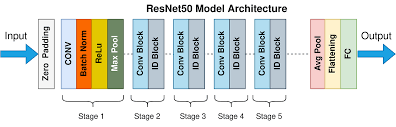
\includegraphics[width=.9\textwidth]{img/resnet.png}
	\caption{Schemat architektury modelu ResNet50}  \label{rys:resnet}
\end{figure}

\subsection*{ConvNeXt}

ConvNeXt to model o nowoczesnej architekturze CNN, który został opracowany w celu integracji najlepszych praktyk z konwolucyjnych sieci neuronowych i nowoczesnych technik pochodzących od transformerów. ConvNeXt wykorzystuje bardziej złożone 
operacje konwolucyjne oraz zaawansowane techniki normalizacji i optymalizacji, co pozwala na osiąganie bardzo dobrych wyników w różnych zadaniach klasyfikacji.

ConvNeXt został zaprojektowany z myślą o zastosowaniu najnowszych technik z dziedziny głębokiego uczenia, takich jak normalizacja warstw (Layer Normalization), mechanizmy uwagi (Attention Mechanisms) oraz bardziej złożone architektury 
warstw konwolucyjnych. W ConvNeXt zastosowano podejście polegające na udoskonaleniu tradycyjnych modułów konwolucyjnych poprzez dodanie elementów inspirowanych transformerami, co prowadzi do lepszej wydajności i efektywności obliczeniowej.

Podstawowym elementem ConvNeXt jest moduł konwolucyjny, który został zoptymalizowany w celu lepszego uchwycenia złożonych wzorców w danych. Architektura ConvNeXt łączy tradycyjne podejścia konwolucyjne z nowymi koncepcjami, co 
prowadzi do lepszej wydajności i efektywności obliczeniowej.

ConvNeXt został wybrany do tego projektu ze względu na swoje nowoczesne podejście i wysoką wydajność w klasyfikacji obrazów, co pozwala na dokładne porównanie z wcześniejszymi modelami state-of-art, takimi jak ResNet.

\subsection*{DeepLabv3}

DeepLabv3 z kolei jest modelem wykorzystywanym do segmentacji obrazów, który został opracowany przez zespół Google. Wykorzystuje on techniki takie jak atrous convolutions (dylatowane konwolucje) i Conditional Random Fields (CRFs), które 
pozwalają na dokładne segmentowanie obiektów na różnych skalach. DeepLabv3+ jest najnowszą wersją tej serii, która łączy atrous convolutions z modulem spatial pyramid pooling, co pozwala na uchwycenie bogatych informacji kontekstowych.

Podstawowym elementem DeepLabv3 jest zastosowanie atrous convolutions, które mogą być opisane równaniem:

\begin{equation}
y[i] = \sum_{k=1}^{K} x[i + r \cdot k] \cdot w[k]
\end{equation}

gdzie \( y[i] \) to wyjście konwolucji, \( x \) to wejście, \( w \) to zestaw wag, \( K \) to rozmiar filtra, a \( r \) 
to współczynnik dylatacji.

Dzięki zastosowaniu atrous convolutions, DeepLabv3 może uchwycić informacje na różnych skalach bez utraty rozdzielczości, co jest kluczowe dla dokładnej segmentacji. Dodatkowo, wykorzystanie spatial pyramid pooling pozwala na 
zbieranie informacji kontekstowych z całego obrazu, co poprawia dokładność segmentacji.

DeepLabv3 został wybrany ze względu na swoją zdolność do precyzyjnej segmentacji obrazów oraz uniwersalnośc użycia, co jest kluczowe dla wyodrębnienia obiektów z tła przed dalszą analizą i klasyfikacją.

\subsection*{Uzasadnienie wyboru modeli}

Wybór ResNet, ConvNeXt oraz DeepLabv3 opierał się na ich sprawdzonej skuteczności w swoich dziedzinach oraz zdolności do realizacji celów tego projektu. ResNet, jako starszy model, pozwala na ocenę wpływu tła na klasyfikację obrazów w 
kontekście bardziej tradycyjnych architektur. ConvNeXt, będący nowoczesnym modelem, reprezentuje najnowsze podejścia i innowacje w dziedzinie głębokiego uczenia, co pozwala na ocenę, jak nowe technologie radzą sobie z problemem tła w porównaniu
do nieco starszych technik. DeepLabv3, jako uniwersalny model segmentacji, umożliwia precyzyjne usunięcie tła, co jest kluczowe dla analiz prowadzonych w ramach tego projektu.

Wykorzystanie gotowych, pretrenowanych modeli pozwoliło skupić się na głównym celu badania – analizie wpływu tła na klasyfikację obrazów – bez konieczności poświęcania czasu na trenowanie modeli od podstaw. Dzięki temu możliwe było 
przeprowadzenie bardziej szczegółowych i kompleksowych badań w zakresie modyfikacji tła i jego wpływu na wydajność modeli klasyfikacyjnych.

\section*{Wybrane metryki}

W celu analizy wyników klasyfikacji przed i po modyfikacjach tła, zastosowano cztery kluczowe metryki: dokładność (accuracy), pewność klasyfikacji (confidence scores), precyzję (precision), recall oraz F1 score. Analizowana będzie również 
macierz korelacji w celu zbadania wzajemnych zależności między modyfikacjami. Metryki te zostały wybrane ze względu na ich zdolność do dostarczania wartościowych informacji na temat wydajności modeli w różnych warunkach, sprawdzają się
one idealnie do wstępnych analiz modeli oraz do oceny jak skutecznie modele radzą sobie z przedstawionym problemem klasyfikacji. Wykorzystane metryki zostaną w tej części krótko opisane. Metryki przeprowadzonych badań będą analizowane 
całościowo, jak również osobno dla każdej klasy, dla każdej różnej modyfikacji tła oraz dla różnych rozmiarów obiektu na obrazie.


\subsection*{Dokładność (Accuracy)}

Dokładność jest jedną z najprostszych i najbardziej intuicyjnych metryk stosowanych do oceny jakości modeli klasyfikacyjnych. Definiuje się ją jako stosunek liczby poprawnie sklasyfikowanych przykładów do całkowitej liczby 
przykładów. Będzie to jedna z głównych analizowanych metryk. Każda klasa będzie posiadała taką samą ilość próbek, także problem interpretowalności tej metryki, jaki występuje przy danych niezbalansowanych nie wystąpi.

Wzór na dokładność prezentuje się następująco:

\begin{equation}
\text{Accuracy} = \frac{TP + TN}{TP + TN + FP + FN}
\end{equation}

gdzie:
\begin{itemize}
    \item TP (True Positives) - liczba prawdziwie pozytywnych przypadków,
    \item TN (True Negatives) - liczba prawdziwie negatywnych przypadków,
    \item FP (False Positives) - liczba fałszywie pozytywnych przypadków,
    \item FN (False Negatives) - liczba fałszywie negatywnych przypadków.
\end{itemize}

Dokładność została wybrana jako podstawowa metryka oceny modeli, ponieważ daje ogólny obraz wydajności modelu.

\subsection*{Precyzja (Precision)}
Precyzja (precision) jest metryką oceniającą dokładność pozytywnych predykcji modelu. Definiuje się ją jako stosunek liczby prawdziwie pozytywnych przypadków do sumy liczby prawdziwie pozytywnych i fałszywie pozytywnych przypadków. 
Wzór na precyzję jest następujący:

\[
\text{Precision} = \frac{TP}{TP + FP}
\]


\subsection*{Recall}
Recall, zwany również czułością lub TPR (True Positive Rate), mierzy zdolność modelu do wykrywania wszystkich pozytywnych przypadków. Jest definiowany jako stosunek liczby prawdziwie pozytywnych przypadków do sumy liczby prawdziwie 
pozytywnych i fałszywie negatywnych przypadków. Wzór na recall 
jest następujący:

\[
\text{Recall} = \frac{TP}{TP + FN}
\]

\subsection*{F1 Score}
F1 score jest harmoniczną średnią precyzji i recall. Jest używany jako pojedyncza metryka oceniająca wydajność modelu, która uwzględnia zarówno precyzję, jak i recall. Wzór na F1 score jest następujący:

\[
\text{F1 Score} = 2 \times \frac{\text{Precision} \times \text{Recall}}{\text{Precision} + \text{Recall}}
\]


\subsection*{Pewność klasyfikacji (Confidence Scores)}

Pewność klasyfikacji (confidence scores) odnosi się do stopnia pewności modelu co do przypisania danego przykładu do określonej klasy. Jest to istotna metryka, ponieważ dostarcza dodatkowych informacji o tym, jak pewny jest model swoich 
predykcji. Wyższe wartości pewności oznaczają większe zaufanie modelu do swojej klasyfikacji.

Analiza pewności klasyfikacji pozwala na ocenę, jak model jest pewny swoich decyzji oraz jak modyfikacje tła wpływają na pewność modeli.

\section*{Opis wykorzystanego zbioru danych}

W ramach niniejszego badania wykorzystano zbiór danych ImageNet1k, który jest jednym z najbardziej rozpoznawalnych i szeroko stosowanych zestawów danych w dziedzinie przetwarzania obrazów i głębokiego uczenia. ImageNet1k składa się z 
obrazów należących do 1000 różnych klas, co pozwala na wszechstronną ocenę wydajności modeli klasyfikacyjnych w różnorodnych scenariuszach.

\subsection*{Struktura zbioru danych}

Zbiór danych ImageNet1k jest podzielony na trzy części: treningową, walidacyjną oraz testową. Każda z tych części ma określoną liczbę obrazów na klasę, co umożliwia wszechstronne trenowanie, walidację i testowanie modeli klasyfikacyjnych.

\begin{itemize}
    \item \textbf{Zbiór treningowy:} Zawiera około 1300 obrazów na klasę, co daje szeroką bazę danych do nauki modeli. 
    Duża liczba obrazów na klasę pozwala na efektywne trenowanie głębokich sieci neuronowych, co prowadzi do lepszego 
    uchwycenia cech charakterystycznych dla każdej klasy.
    \item \textbf{Zbiór walidacyjny:} Składa się z 50 obrazów na klasę. Zbiór walidacyjny jest używany do monitorowania 
    wydajności modelu w trakcie treningu i do wczesnego wykrywania problemów takich jak nadmierne dopasowanie 
    (overfitting).
    \item \textbf{Zbiór testowy:} Zawiera 100 obrazów na klasę. Zbiór testowy służy do ostatecznej oceny wydajności 
    modeli po zakończeniu procesu treningu i walidacji.
\end{itemize}

\subsection*{Różnorodność obrazów}

Obrazy w zbiorze ImageNet1k charakteryzują się różnorodnością rozdzielczości oraz warunków, w jakich zostały wykonane. Inaczej mówiąć, oznacza to, że obrazy mogą przedstawiać obiekty w różnych skalach, oświetleniach, perspektywach i na 
różnych tłach. Taka różnorodność sprawia, że zbiór ImageNet1k doskonale odzwierciedla realistyczne warunki, z jakimi modele mogą się spotkać w praktycznych zastosowaniach. Dzięki temu, modele trenowane na tym zbiorze danych są bardziej 
uniwersalne i mają lepszą zdolność do generalizacji. 

\subsection*{Popularność i znaczenie ImageNet1k}

ImageNet1k jest jednym z najczęściej używanych zestawów danych w badaniach nad różnymi problemami związanymi z głębokim uczeniem, co jest wynikiem jego dużej ilośći zdjęć, różnorodności i realistycznego charakteru. Wiele przełomowych modeli, 
takich jak VGG czy ResNet, zostało przetestowanych i zweryfikowanych przy użyciu tego zestawu danych. Popularność ImageNet1k sprawia, że wyniki uzyskane na tym zbiorze są łatwo porównywalne z wynikami innych badań, co umożliwia ocenę 
postępów i łatwe porównywanie z innymi badaczami.


\section*{Plan badań}

Niniejszy rozdział opisuje szczegółowy plan badań, które zostały przeprowadzone w celu zbadania wpływu tła na klasyfikację obrazów zwierząt. Poniżej szczegółowo przedstawiono kroki podjęte w celu realizacji badań.

\subsection*{Przygotowanie środowiska pracy}

Pierwszym krokiem było przygotowanie odpowiedniego środowiska pracy. W tym celu skonfigurowano środowisko programistyczne, które obejmowało instalację niezbędnych bibliotek i narzędzi, takich jak numpy, pandas, scikit-learn, 
PIL, matplotlib, seaborn, torch oraz torchvision. Przyogotowano również wirtualne środowisko, pobrano dane z oficjalnej strony ImageNet. 

\subsection*{Implementacja}

Całość implementacji została wykonana w języku Python, który dzięki swojej elastyczności i szerokiej gamie bibliotek doskonale nadaje się do realizacji złożonych projektów związanych z uczeniem maszynowym. Większość funkcjonalności została 
zaimplementowana w formie samodzielnych skryptów, podczas gdy same badania, czyli opracowywanie wyników, są dostępne w formie interaktywnych notebooków Jupyter. Taki podział pozwala na łatwe uruchamianie skryptów oraz jednoczesną analizę i 
wizualizację wyników.

Skrypty są nazwane zgodnie ze swoją funkcjonalnością, co ułatwia nawigację i zrozumienie ich przeznaczenia. Każdy skrypt zawiera funkcje z dobrze opisanymi nazwami, a każda funkcja posiada docstringi, które szczegółowo wyjaśniają jej działanie.

Dodatkowo, cała implementacja wraz z dokładnym opisem znajduje się na GitHubie, gdzie można znaleźć pełen kod oraz plik README zawierający instrukcje dotyczące uruchamiania skryptów i analizy wyników. 

Link do repozytorium GitHub: \href{https://github.com/paulpel/BackgroundImpactAnalysis}{link do repozytorium}

\subsection*{Wybranie modeli do segmentacji i klasyfikacji}

Kolejnym ważnym krokiem było zaplanowanie wykorzystywanych modeli w badaniu. Do segmentacji obrazów wybrano model DeepLabv3, który jest zaawansowanym modelem segmentacji zdolnym do precyzyjnego wyodrębniania obiektów z tła. 
Do klasyfikacji obrazów wybrano dwa modele: ResNet, reprezentujący starszą generację modeli głębokiego uczenia, oraz ConvNeXt, będący nowszym i bardziej zaawansowanym modelem. Wybór tych modeli pozwolił na dokładne porównanie ich wydajności 
w kontekście różnych modyfikacji tła oraz dwóch genereacji modeli.

\subsection*{Wybranie klas zwierząt}

Ze względu na ograniczoną dostępność klas w modelu segmentacyjnym DeepLabv3, oraz braku zasobów do analizy wszystkich klas, do badań wybrano 10 zróżnicowanych klas zwierząt. Wybrane klasy były takie, które można skutecznie wysegmentować przy 
użyciu tego modelu. Każda klasa ma przynajmniej jedną zbliżoną do siebie, w celu stworzenia warunków badania sprzyjajązych popełnianiu błędów przez klasyfikatory, przykładowo wybrano trzy rasy psów. Przykładowe zdjęcia dla każdej wybranej 
klasy można zaobserwować na Rys. \ref{rys:classes}

\begin{figure}
	\centering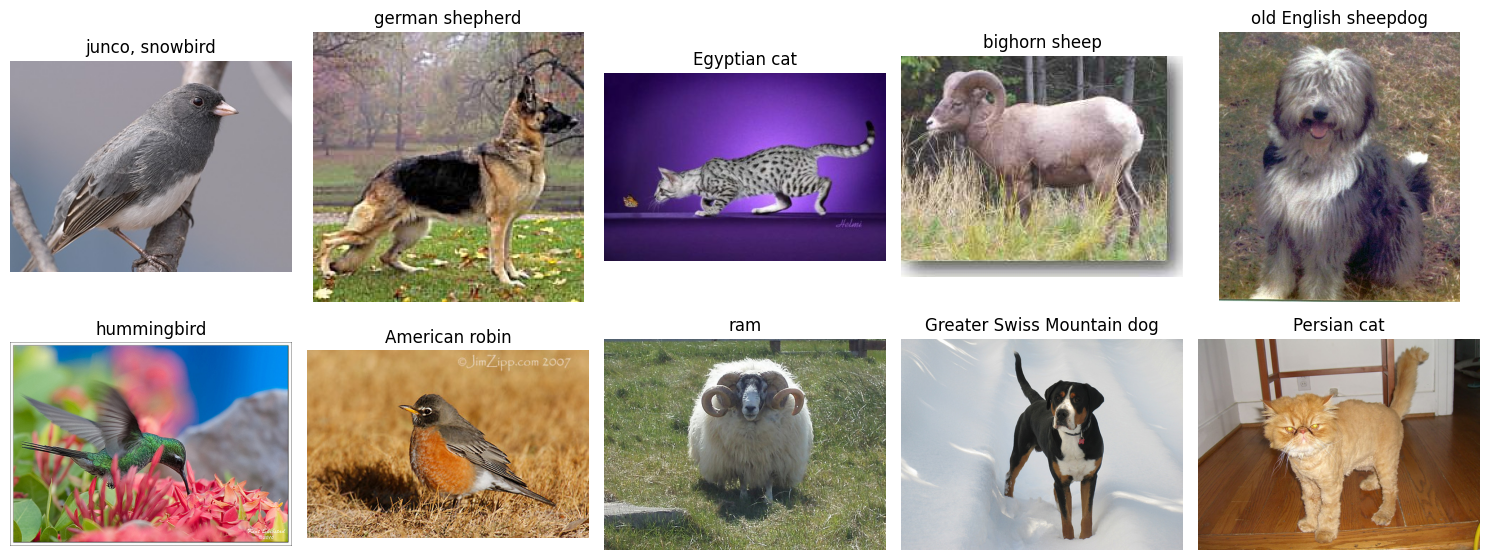
\includegraphics[width=.9\textwidth]{img/classes}
	\caption{Przykładowe oryginalne zdjęcia wybranych klas}  \label{rys:classes}
\end{figure}

\subsection*{Segmentacja obrazów}

Dla każdej z wybranych klas zwierząt wysegmentowano 1000 zdjęć ze zbioru treningowego za pomocą modelu DeepLabv3. Ponieważ na niektórych zdjęciach widniało więcej klas obiektów rozpoznawanych przez ten model, konieczne było zidentyfikowanie 
wartości grayscale dla pożądanej maski obiektu. W tym celu zastosowano skrypt analizujący najczęściej występującą wartość na przestrzeni wszystkich zdjęć dla danej klasy, co pozwoliło na dokładne wyodrębnienie obiektów. Maski zostały zapisane 
do dalszych analiz. Przykładowe uzyskane maski można zaobserwować na Rys. \ref{rys:masks}

\begin{figure}
	\centering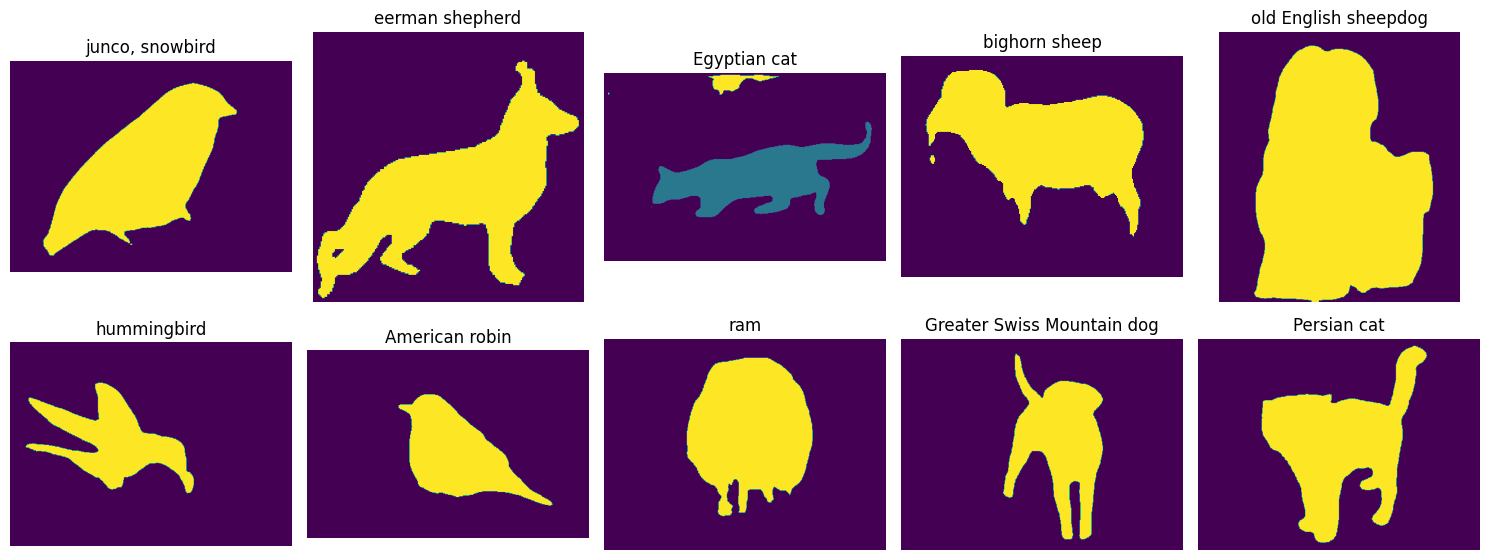
\includegraphics[width=.9\textwidth]{img/masks}
	\caption{Maski przykładowych wysegmentowanych obrazów}  \label{rys:masks}
\end{figure}

\subsection*{Przygotowanie zmodyfikowanych zbiorów zdjęć}

Dla każdej klasy zwierząt przygotowano różne zestawy zmodyfikowanych zdjęć:
\begin{itemize}
    \item \textbf{Zdjęcia z samym obiektem:} Usunięto tło za pomocą maski, pozostawiając czarne tło.
    \item \textbf{Zdjęcia z samym tłem:} Odwrotna modyfikacja do poprzedniej, pozostawiając samo tło bez obiektu. 
    \item \textbf{Przeniesienie obiektu na różne scenerie:} Obiekty zostały przeniesione na inne różne tła o innej scenerii, były to: miasto, pustynia, wnętrze domu, dżungla, góry, niebo, śnieg oraz woda. Ma to na celu stworzenie wariantów 
    zdjęć w innych sceneriach co może być mylące dla klasyfikatorów, szczegónie przy klasyfikacji zwierząt, gdzie podobnie wyglądające gatunki mogą występować w różnych środowiskach. 
    \item \textbf{Zastąpienie tła kolorem o niskim oraz wysokim kontraście do obiektu:} Kolejną modyfikacją było przeniesienie obiektów na tło o kolorze niskokontrastowym oraz wysokokontrastowym. W celu znalezienia tych kolorów, dla każdej klasy 
    przeanalizowano każde zdjęcie i zebrano dominujące kolory dla danej klasy. Następnie przy pomocy specjalnego skryptu wyliczono kolory o niskim i wysokim kontraście do tych obiektów. 
\end{itemize}

Przykładowe zdjęcie, wraz z jego modyfikacjami można zobaczyć na Rys. \ref*{rys:modified}

Modyfikacji dokonywano za pomocą wcześniej uzyskanych masek, dla każdego rodzaju modyfikacji stworzono osobny skrypt w celu zachowania obiektowego charakteru środowiska programistycznego.

\begin{figure}
	\centering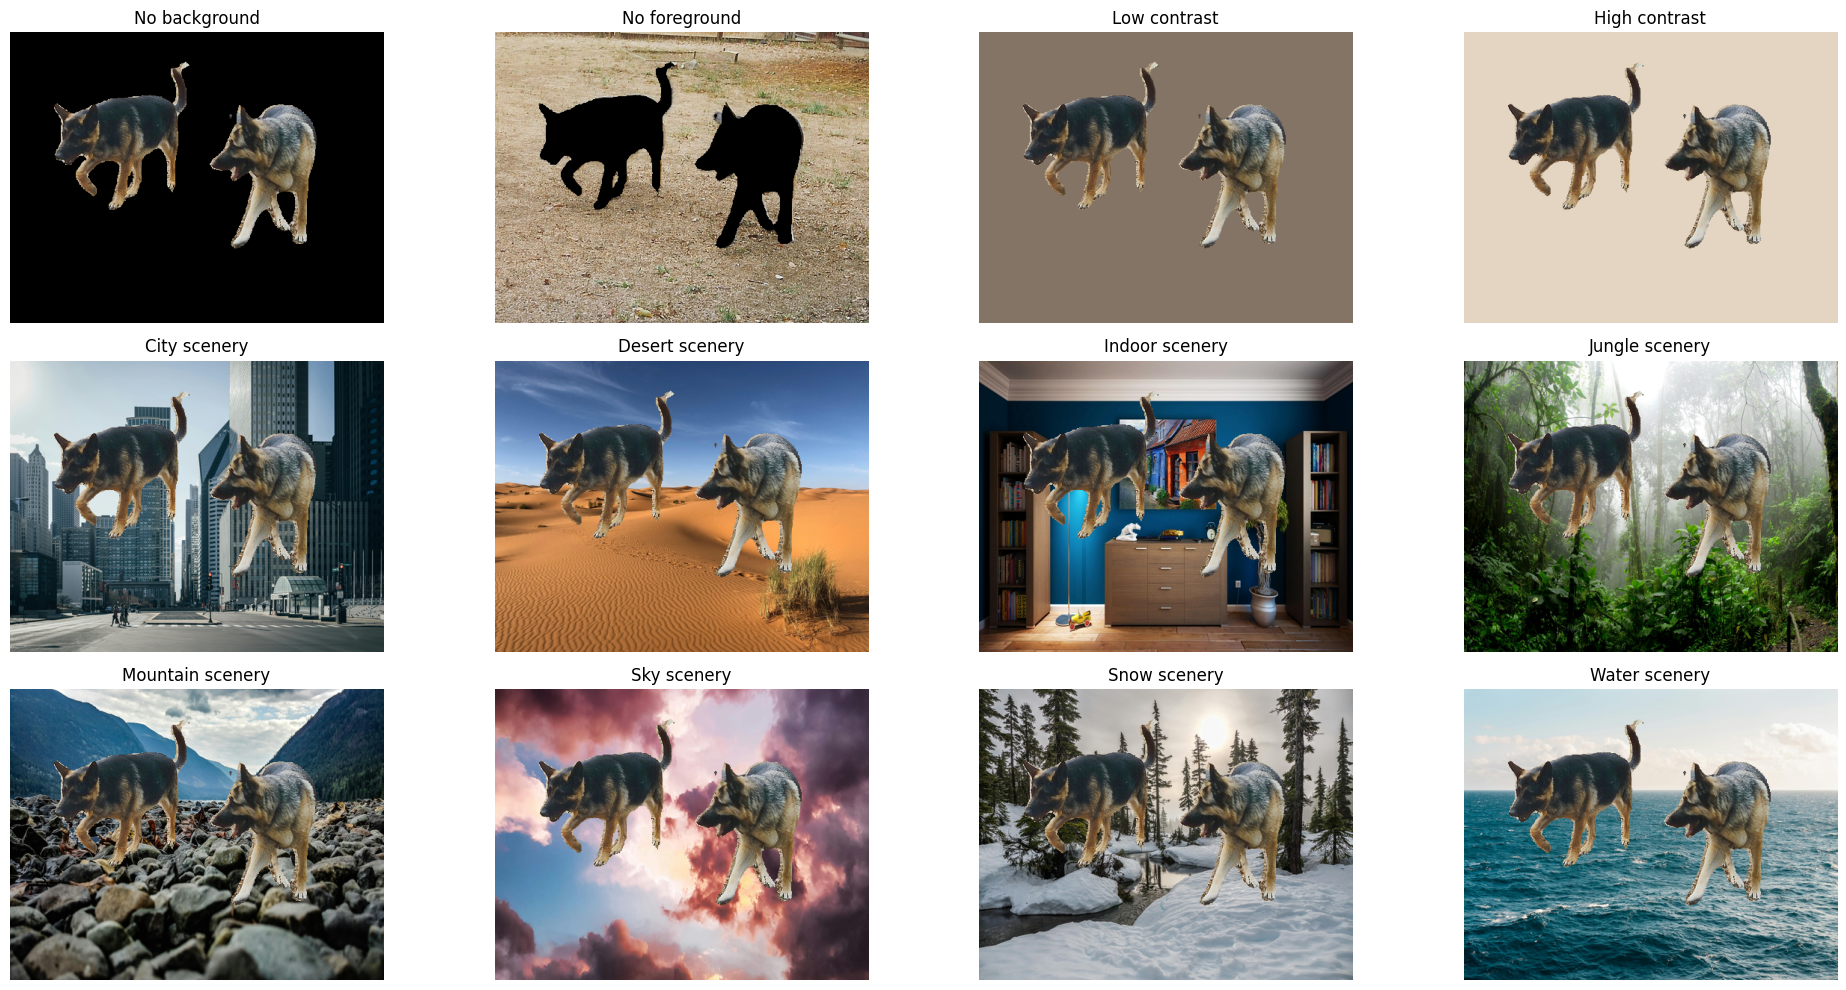
\includegraphics[width=.9\textwidth]{img/modified}
	\caption{Przykładowe zdjęcie poddane modyfikacją}  \label{rys:modified}
\end{figure}

\subsection*{Dokonanie predykcji na wybranych modelach}

Dla każdego zdjęcia dokonano predykcji dla dwóch wybranych modeli, za równo dla oryginalnych zdjęć oraz dla każdego typu modyfikacji. Co dawało dla jednej klasy trzynaście tysięcy predykcji, dwanaście modyfikacji po 1000 zdjęć oraz 
1000 oryginalnych zdjęć. Wyniki predykcji oraz wartości confidence score zapisano w pliku csv.

\subsection*{Dodanie kategorii zdjęć pod względem procentu zajmowanego przez obiekt na zdjęciu}

Zbadanie stosunku wielkości obiektu do całego zdjęcia jest istotne w kontekście badania wpływu tła na klasyfikację, ponieważ może znacząco wpływać na wyniki modeli klasyfikacyjnych. Wielkość obiektu w stosunku do tła może determinować, 
jak łatwo model jest w stanie rozpoznać i sklasyfikować obiekt. Mniejsze obiekty mogą być trudniejsze do wykrycia i bardziej podatne na zakłócenia ze strony tła, podczas gdy większe obiekty mogą dominować obraz, co ułatwia ich klasyfikację. 
Analiza wpływu różnych procentyli wielkości obiektu pozwala na zrozumienie, w jakim stopniu tło oddziałuje na modele w zależności od proporcji obiektu na zdjęciu, co z kolei może prowadzić do bardziej efektywnych strategii przetwarzania i 
klasyfikacji obrazów w praktycznych zastosowaniach.

Dla każdego zdjęcia dodano kategorię pod względem procentu zajmowanego przez obiekt na zdjęciu. Przykładowe zdjęcia o różnych 
rozmiarach obiektów można zobaczyć na Rys. \ref*{rys:size_comp}

\begin{enumerate}
    \item \textbf{Obliczenie powierzchni obiektu:} Dla każdego obrazu obliczono liczbę pikseli zajmowanych przez obiekt.
    \item \textbf{Obliczenie powierzchni całkowitej obrazu:} Liczba pikseli całego obrazu.
    \item \textbf{Obliczenie procentu powierzchni zajmowanej przez obiekt:} Procent powierzchni zajmowanej przez obiekt obliczono za pomocą wzoru:
    \begin{equation}
    \text{Procent powierzchni zajmowanej przez obiekt} = \left( \frac{\text{Powierzchnia obiektu}}{\text{Powierzchnia całkowita obrazu}} \right) \times 100
    \end{equation}
    \item \textbf{Podział obiektów na percentyle:} Obrazy posortowano według procentu powierzchni zajmowanej przez obiekt i 
    podzielono na trzy grupy według wartości percentyli (0,33 oraz 0,66) i nadano każdemu zdjęciu odpowiednią kategorie (SMALL, MEDIUM albo LARGE)
\end{enumerate}

\begin{figure}
	\centering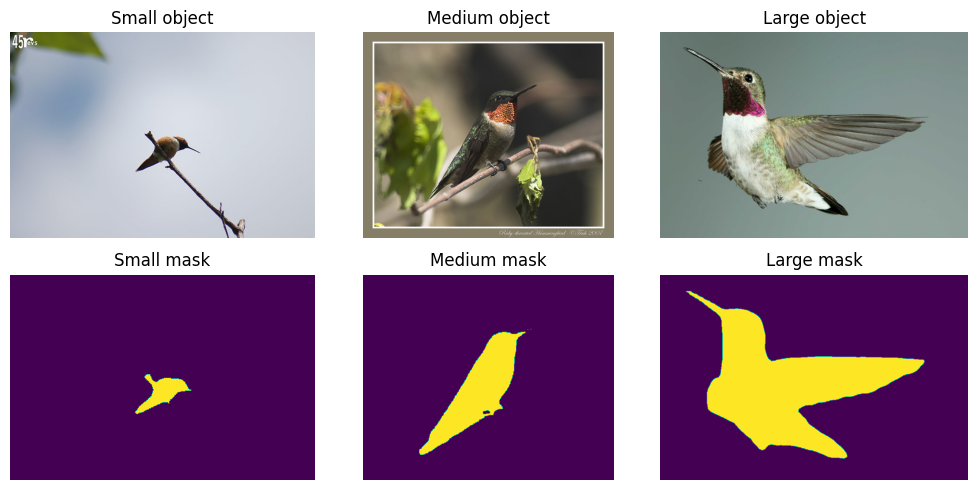
\includegraphics[width=.9\textwidth]{img/size_comp}
	\caption{Przykładowe zdjęcia o różnych rozmiarach obiektów dla klasy "hummingbird"}  \label{rys:size_comp}
\end{figure}

\subsection*{Analiza wyników}

Wygenerowany plik csv załadowano do dataframe, następnie przygotowoną tą ramkę w celu dalszych analiz. Dodano informacje o prawdziwej klasie do każdego zdjęcia oraz informacje True, False w zależnośći od poprawności klasyfikacji dla każdej 
modyfikacji. Ułatwiło to dalsze generowanie statystyk i metryk. Analizy wyników dokonano ze względu na różne czynniki, wymienione poniżej:
\begin{itemize}
    \item \textbf{Analiza ogólna wyników:} Ogólna wydajność modeli na całym zbiorze danych.
    \item \textbf{Analiza pod kątem wielkości obiektu:} Wydajność modeli w zależności od wielkości obiektu na zdjęciu.
    \item \textbf{Analiza pod kątem rodzaju modyfikacji:} Wydajność modeli w zależności od typu modyfikacji tła.
    \item \textbf{Analiza pod kątem klasy:} Wydajność modeli dla każdej klasy zwierząt osobno.
\end{itemize}

\subsection*{Wnioski i dalsze kierunki rozwoju}

Kolejnym etapem badania było wyciągniecie wniosków na podstawie uzyskanych rezultatów oraz przedstawienie potencjalnych kierunków rozwoju projektu.


\chapter*{Badania}

Celem tego rozdziału jest przeprowadzenie analizy wyników klasyfikacji obrazów zwierząt dla modeli ResNet i 
ConvNeXt. Analiza obejmuje porównanie skuteczności modeli w różnych scenariuszach modyfikacji tła oraz w zależności 
od wielkości obiektu na obrazie. Przeanalizowane zostaną ogólne metryki, wyniki dla poszczególnych klas oraz wpływ 
wielkości obiektu na dokładność klasyfikacji.


\begin{table}
	\centering
	\begin{tabular}{|c|c|c|c|c|c|}
		\hline
		\textbf{Model} & \textbf{Type} & \textbf{Accuracy} & \textbf{Precision} & \textbf{Recall} & \textbf{F1-score} \\
		\hline
		ResNet & Original & 0.886500 & 0.967026 & 0.886500 & 0.922742 \\
		\hline
		ResNet & Modified & 0.697018 & 0.948539 & 0.697018 & 0.802350 \\
		\hline
		ConvNeXt & Original & 0.943300 & 0.972519 & 0.943300 & 0.956791 \\
		\hline
		ConvNeXt & Modified & 0.790873 & 0.961080 & 0.790873 & 0.866282 \\
		\hline
	\end{tabular}
	\caption{Metryki porównawcze modeli ResNet i ConvNeXt}
	\label{tab:model_comparison_metrics}
\end{table}

\begin{figure}
	\centering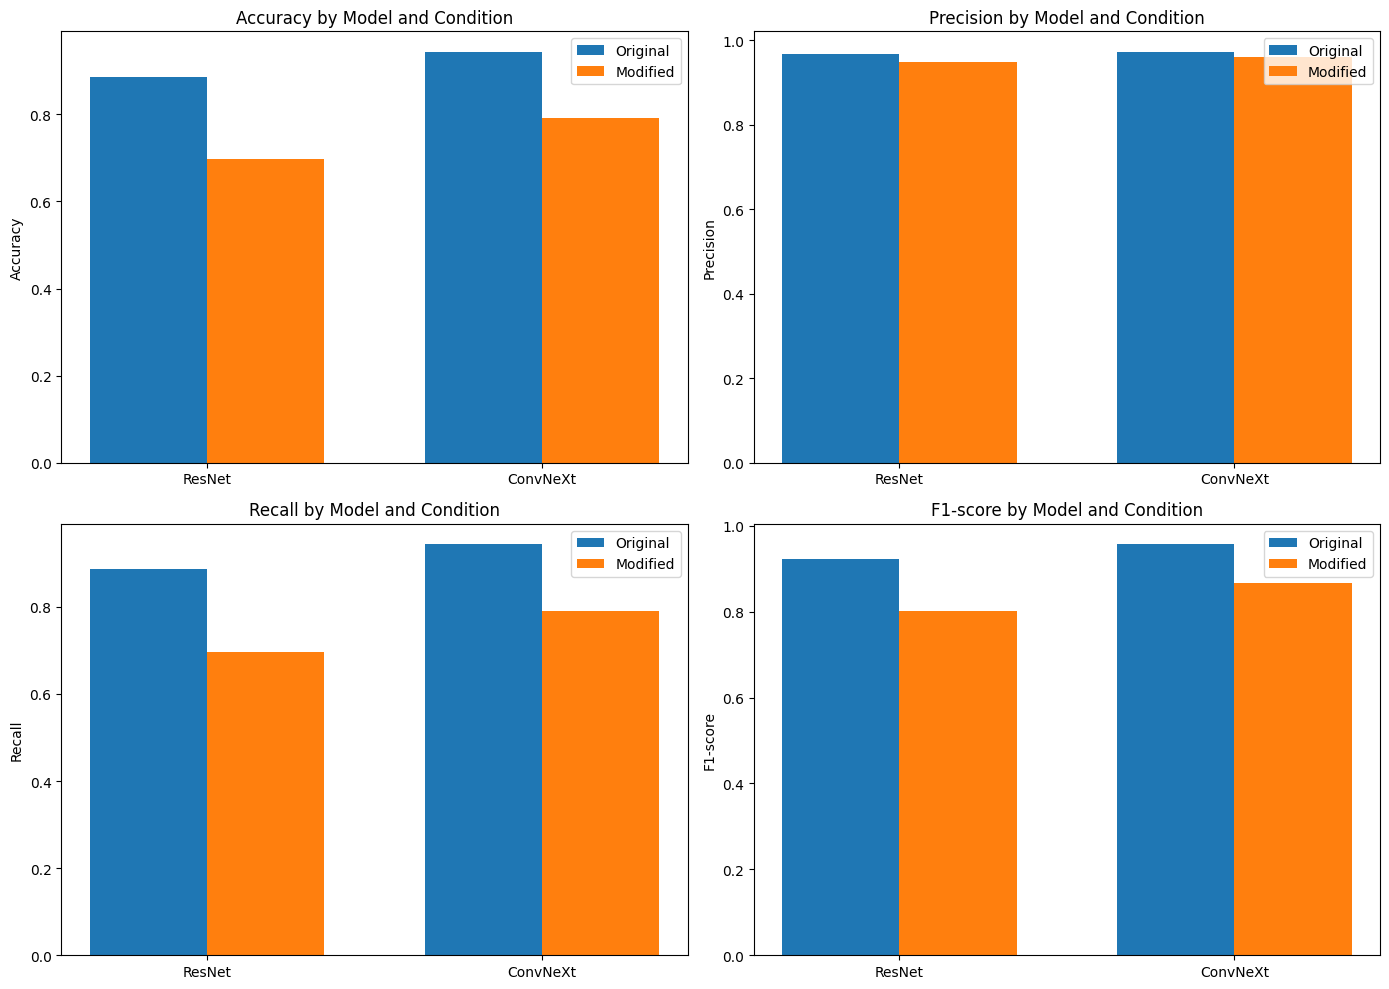
\includegraphics[width=.9\textwidth]{img/overall_metrics}
	\caption{Metryki dla danych oryginalnych zestawionych z danymi o zmodyfikowanych tłach}  
    \label{rys:overall_metrics}
\end{figure}

\begin{table}
	\centering
	\begin{tabular}{|c|c|c|c|c|c|}
		\hline
		\textbf{Model} & \textbf{Type} & \textbf{Average} & 
		\textbf{Average correct} & \textbf{Average incorrect} \\
		\hline
		ResNet & Original & 85.188854 & 89.137424 & 54.348263 \\
		\hline
		ResNet & Modified & 71.694490 & 83.929904 & 43.546579  \\
		\hline
		ConvNeXt & Original & 85.188854 & 89.137424 & 54.348263 \\
		\hline
		ConvNeXt & Modified & 71.694490 & 83.929904 & 43.546579 \\
		\hline
	\end{tabular}
	\caption{Confidence scores dla modeli ResNet i ConvNeXt}
	\label{tab:model_confidence}
\end{table}

\begin{figure}
	\centering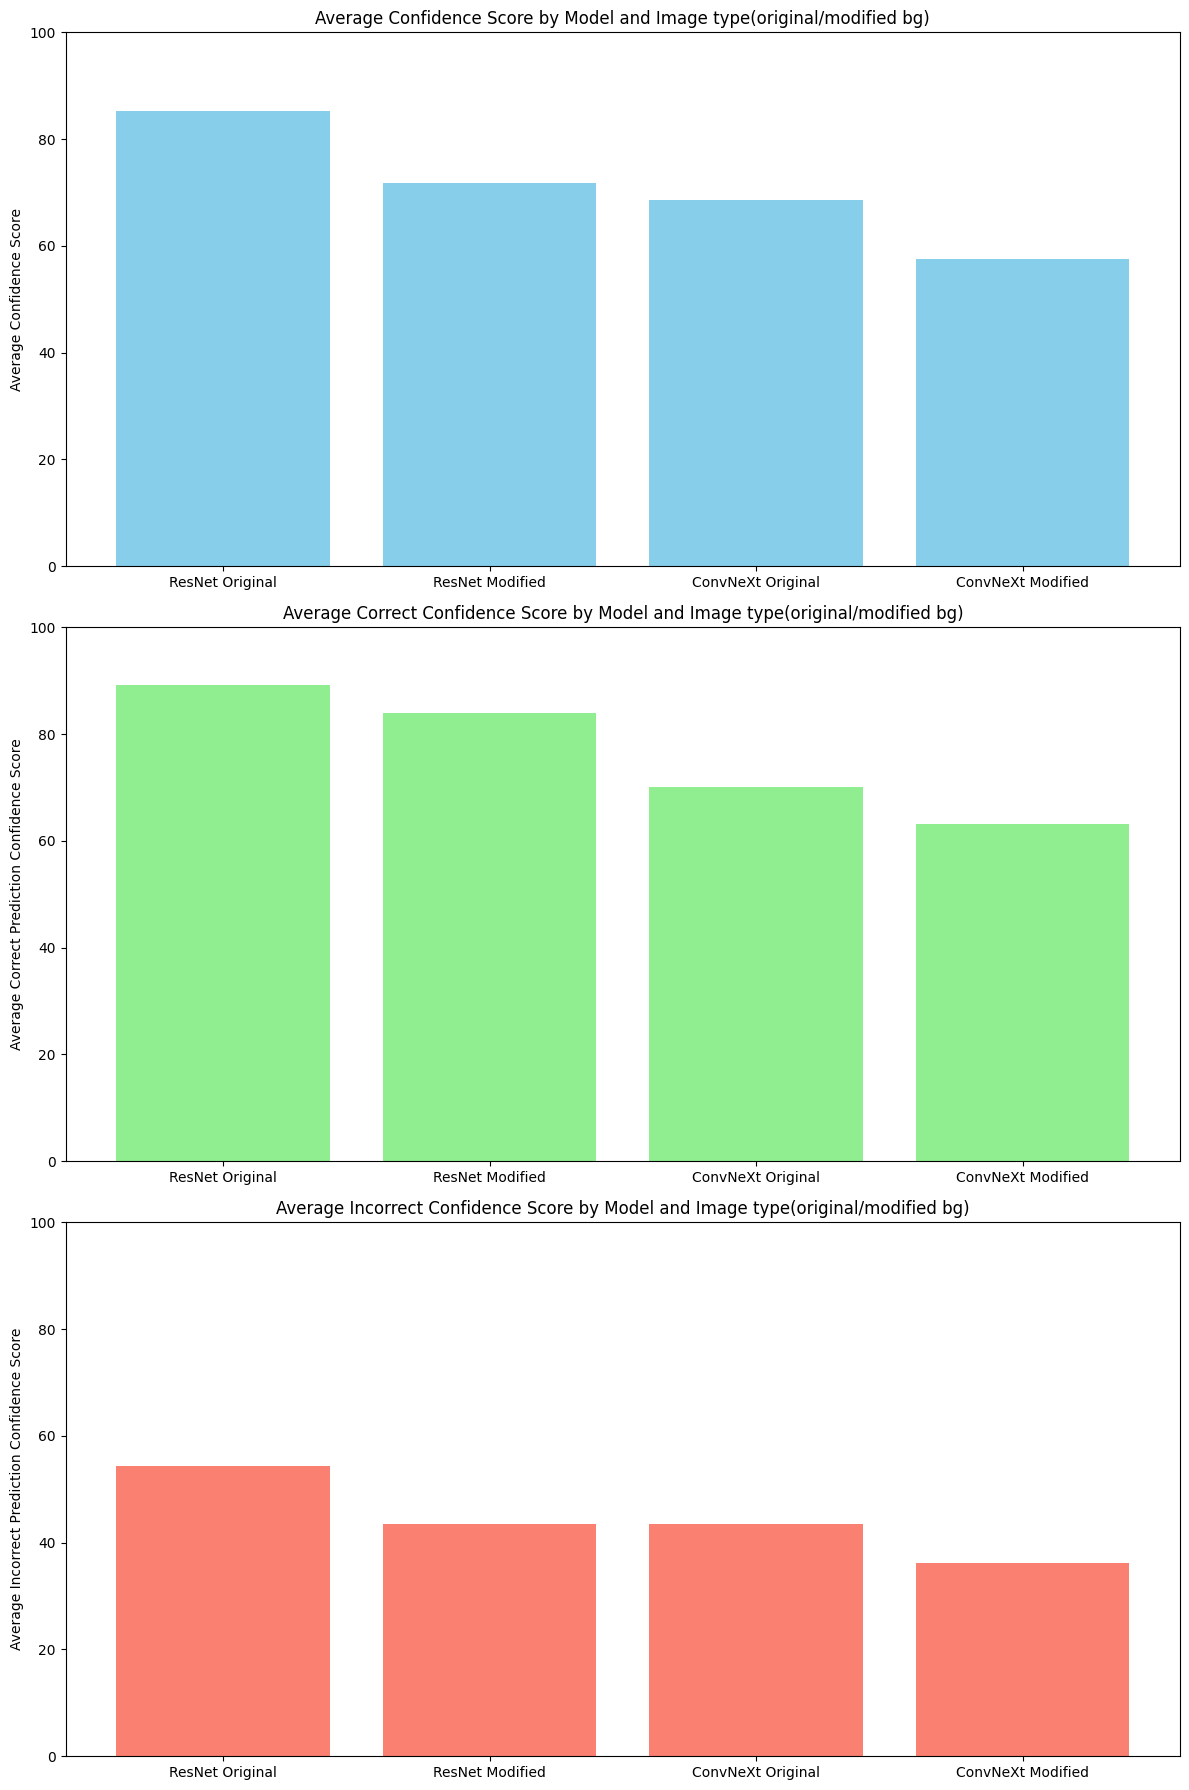
\includegraphics[width=.9\textwidth]{img/confidence_avg}
	\caption{Średnie wartości dla confidence scores}  
    \label{rys:confidence_avg}
\end{figure}

\begin{figure}
	\centering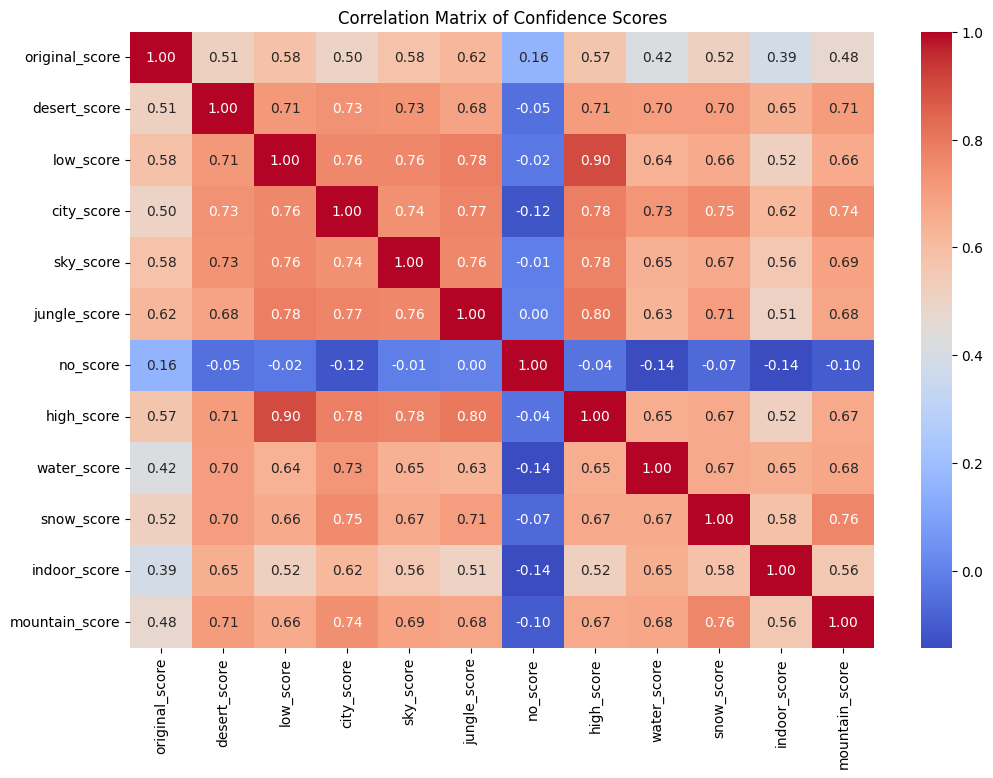
\includegraphics[width=.9\textwidth]{img/correlation_matrix_res}
	\caption{Correlation matrix ResNet confidence}  
    \label{rys:correlation_resnet}
\end{figure}

\begin{figure}
	\centering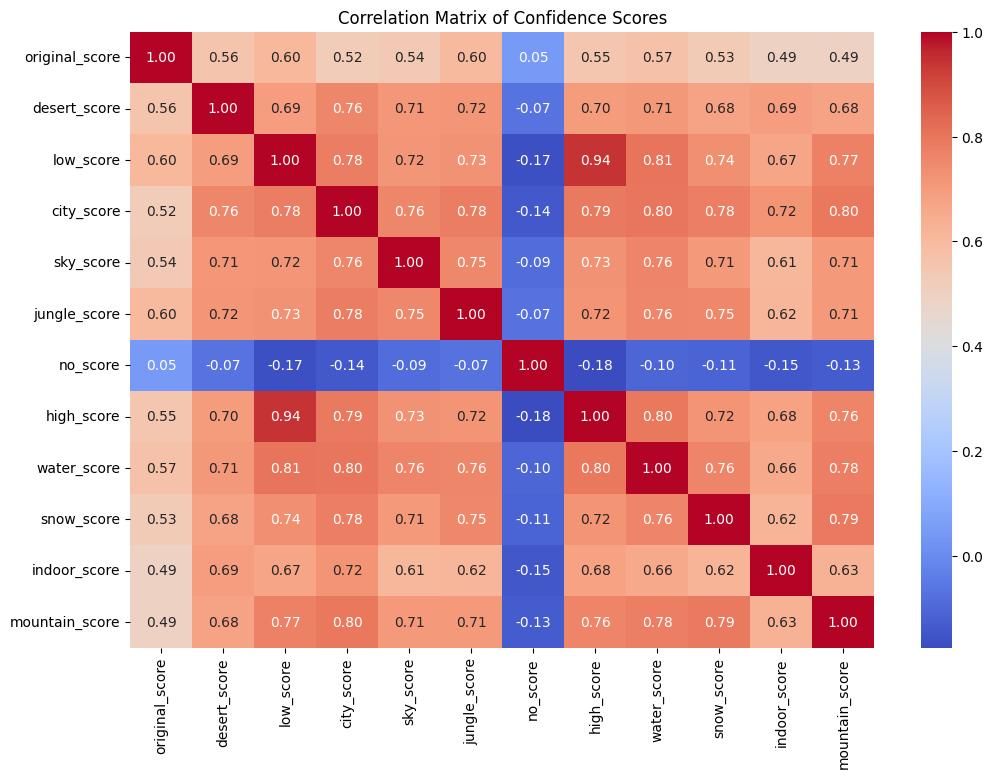
\includegraphics[width=.9\textwidth]{img/correlation_matrix_conv}
	\caption{Correlation matrix ConvNeXt confidence}  
    \label{rys:correlation_convnext}
\end{figure}

\begin{figure}
	\centering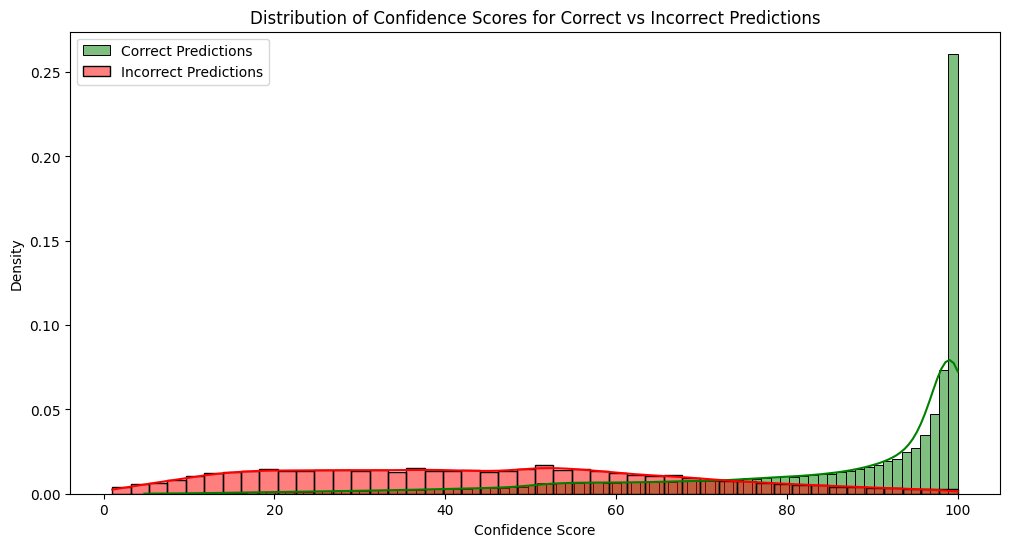
\includegraphics[width=.9\textwidth]{img/resnet_conf_distro}
	\caption{Dystrybucja confidence score dla ResNet}
	\label{rys:res_c_distro}
\end{figure}

\begin{figure}
	\centering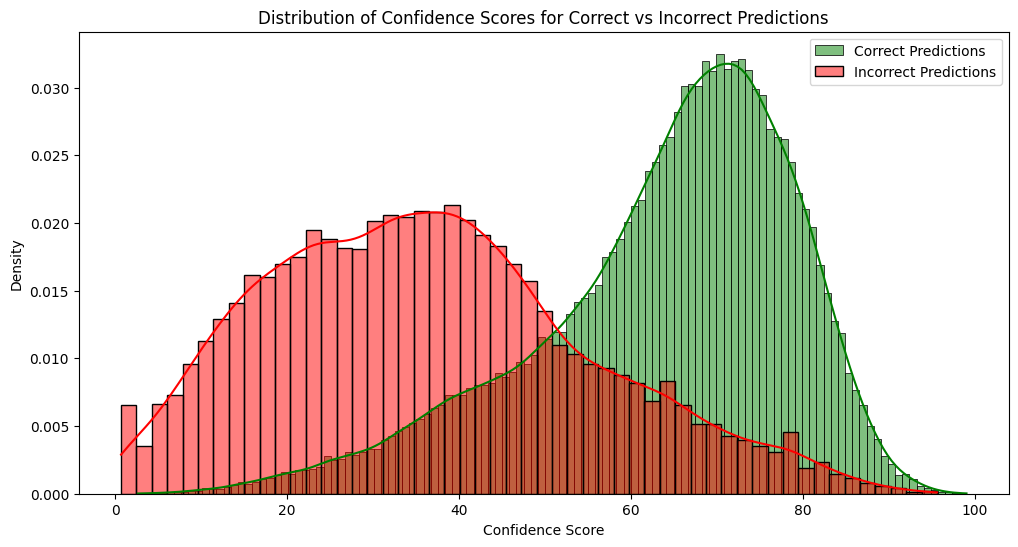
\includegraphics[width=.9\textwidth]{img/convnext_conf_distro}
	\caption{Dystrybucja confidence score dla ConvNext}
	\label{rys:conv_c_distro}
\end{figure}

\begin{figure}
	\centering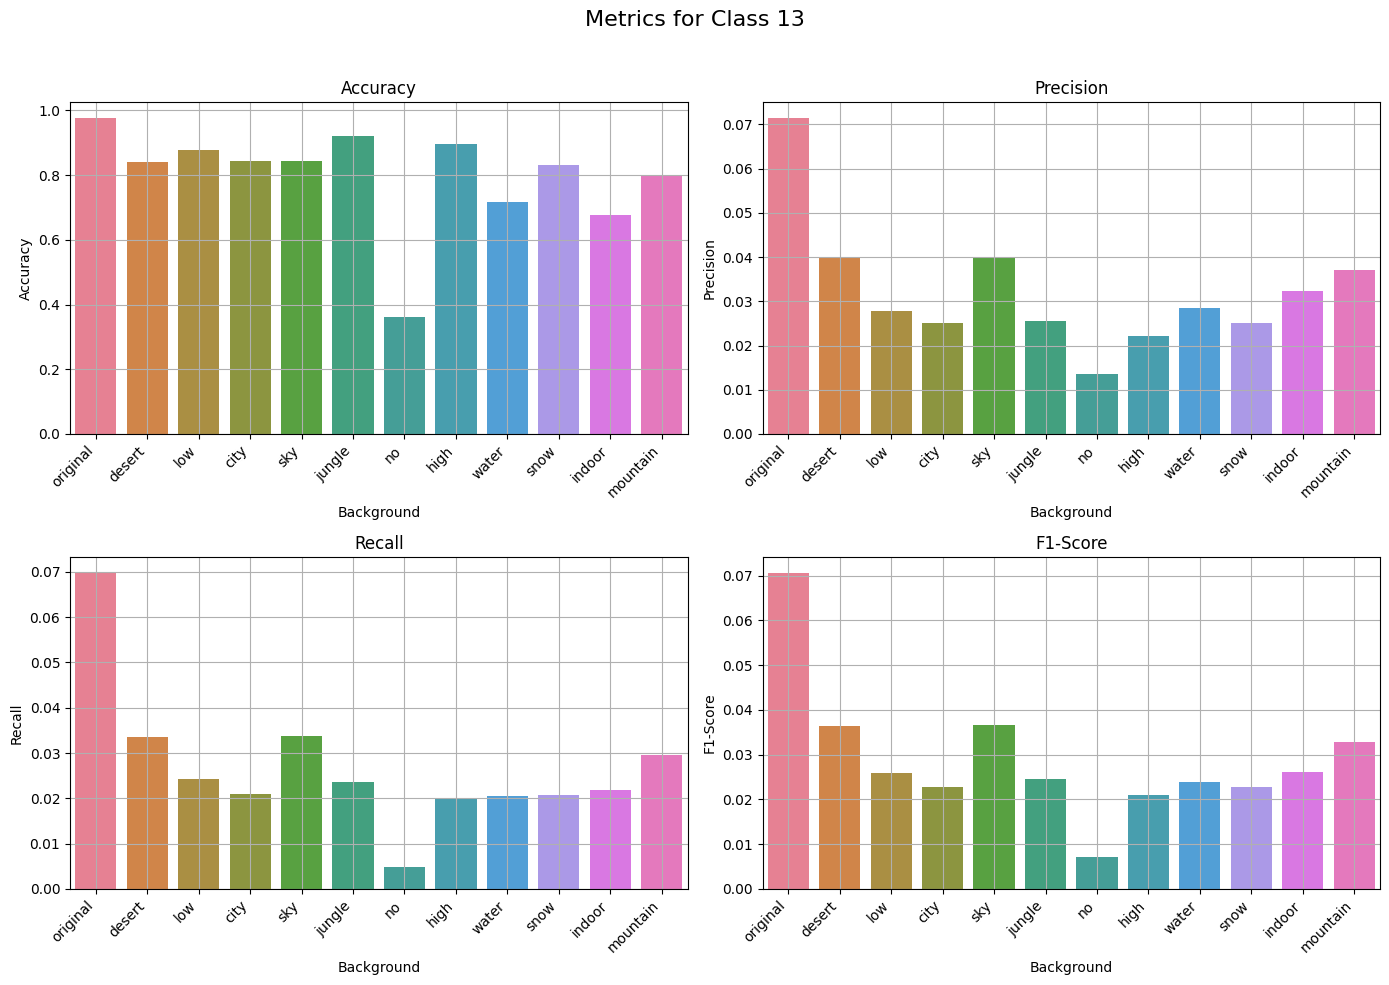
\includegraphics[width=.9\textwidth]{img/13}
	\caption{Metryki}
	\label{rys:13}
\end{figure}

\begin{figure}
	\centering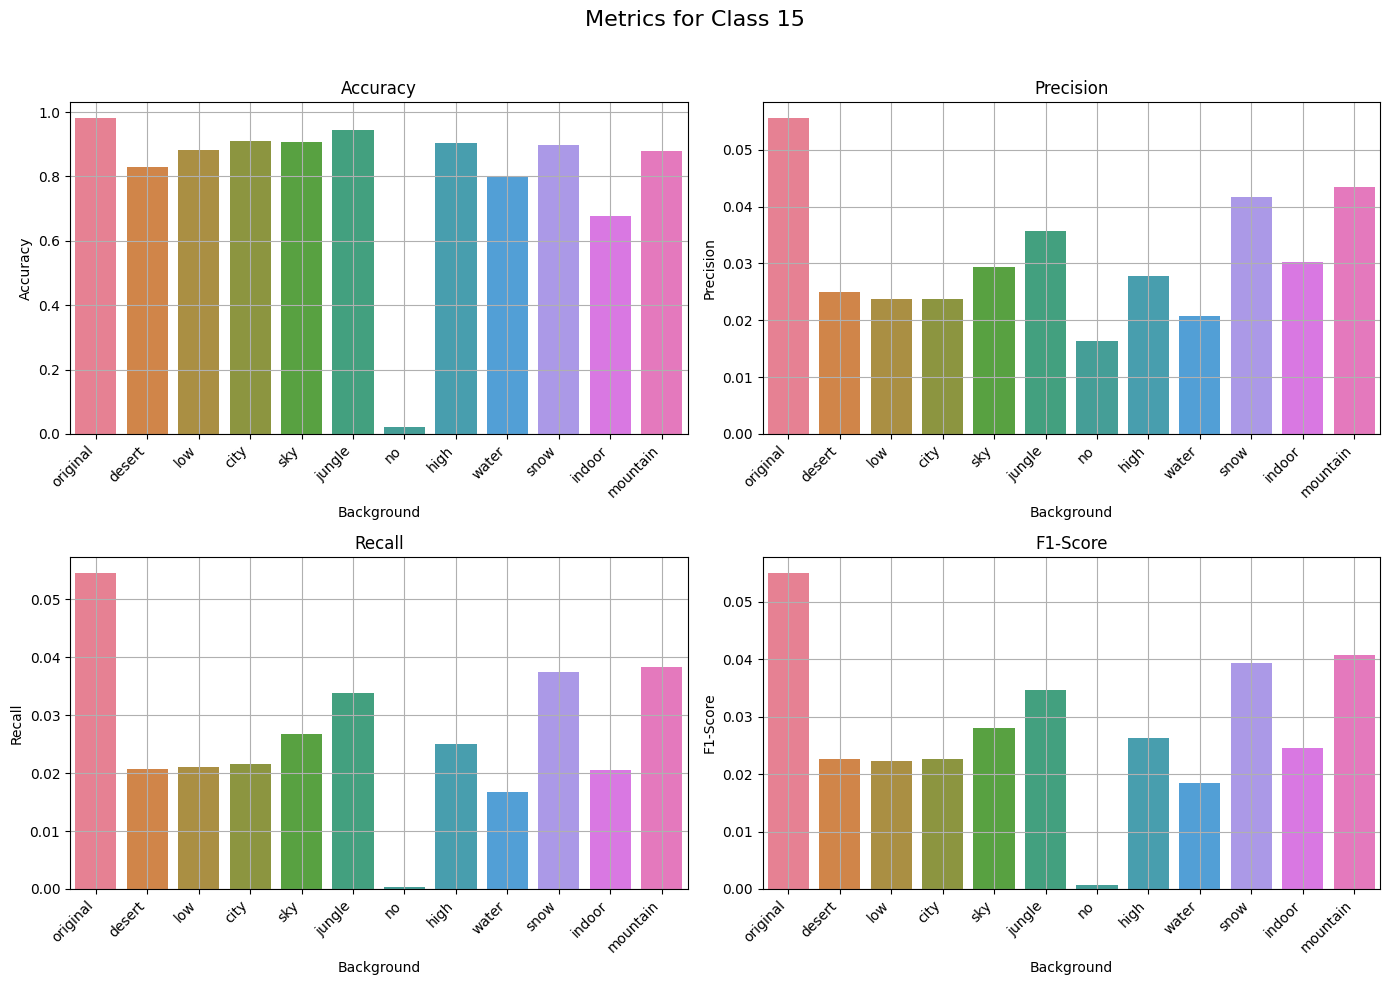
\includegraphics[width=.9\textwidth]{img/15}
	\caption{Metryki}
	\label{rys:15}
\end{figure}

\begin{figure}
	\centering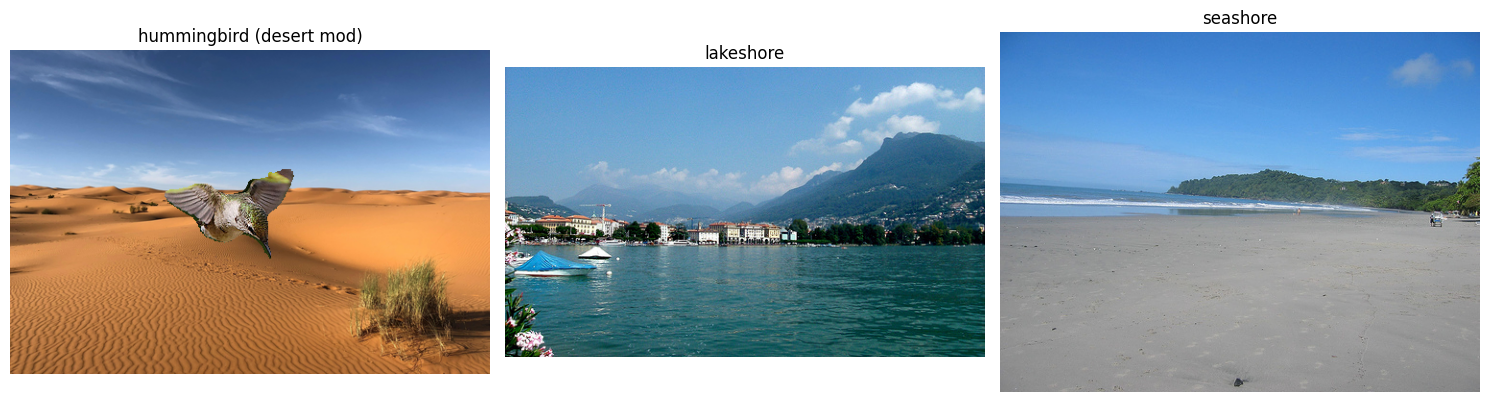
\includegraphics[width=.9\textwidth]{img/94}
	\caption{Metryki}
	\label{rys:94}
\end{figure}

\begin{figure}
	\centering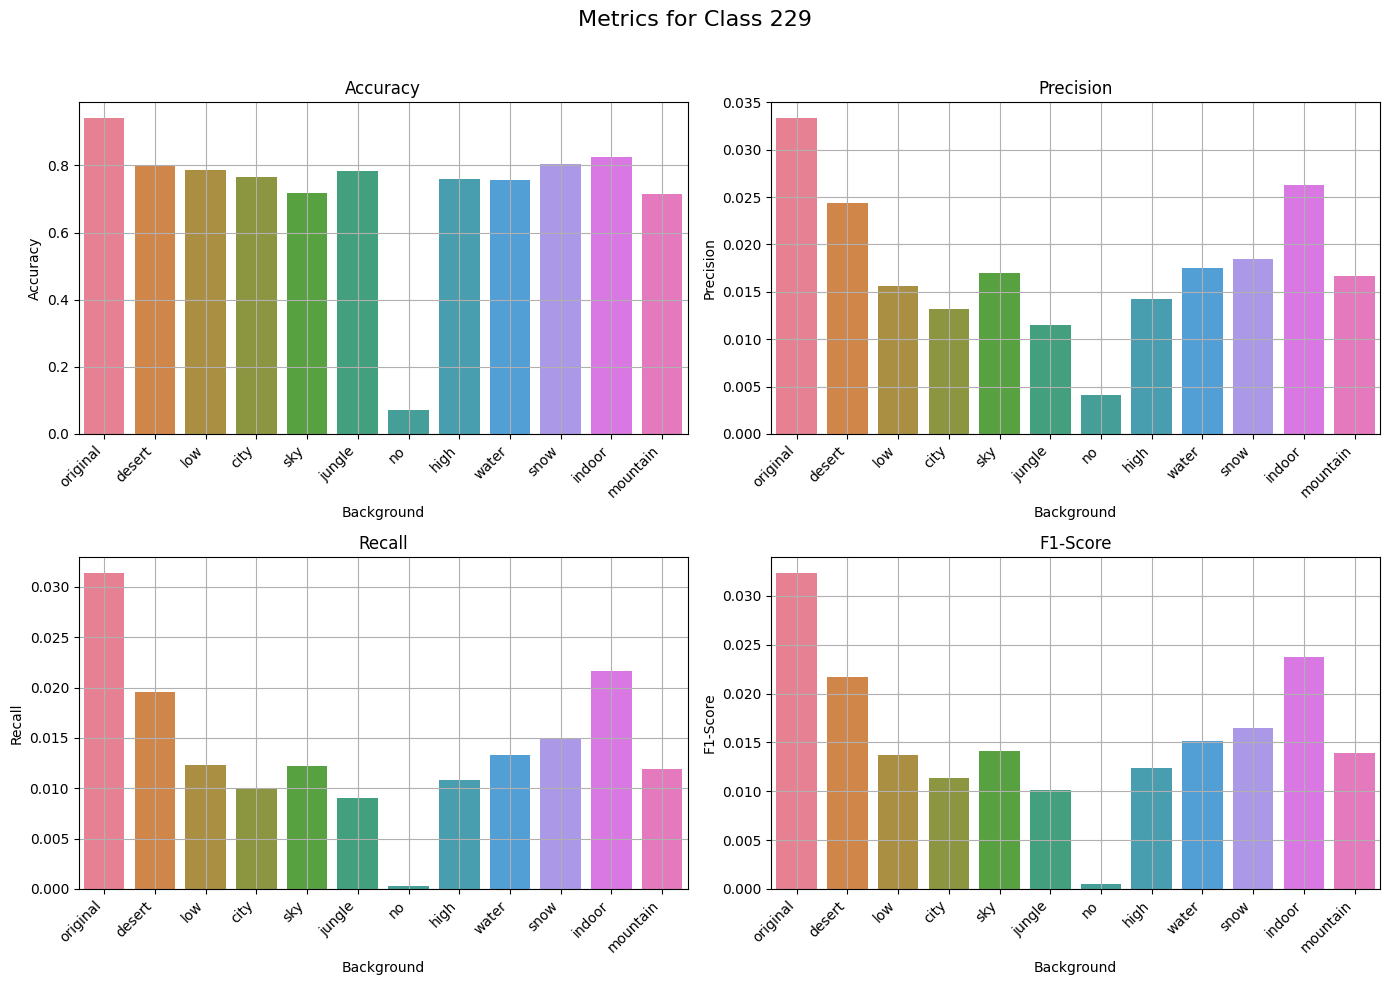
\includegraphics[width=.9\textwidth]{img/229}
	\caption{Metryki}
	\label{rys:229}
\end{figure}

\begin{figure}
	\centering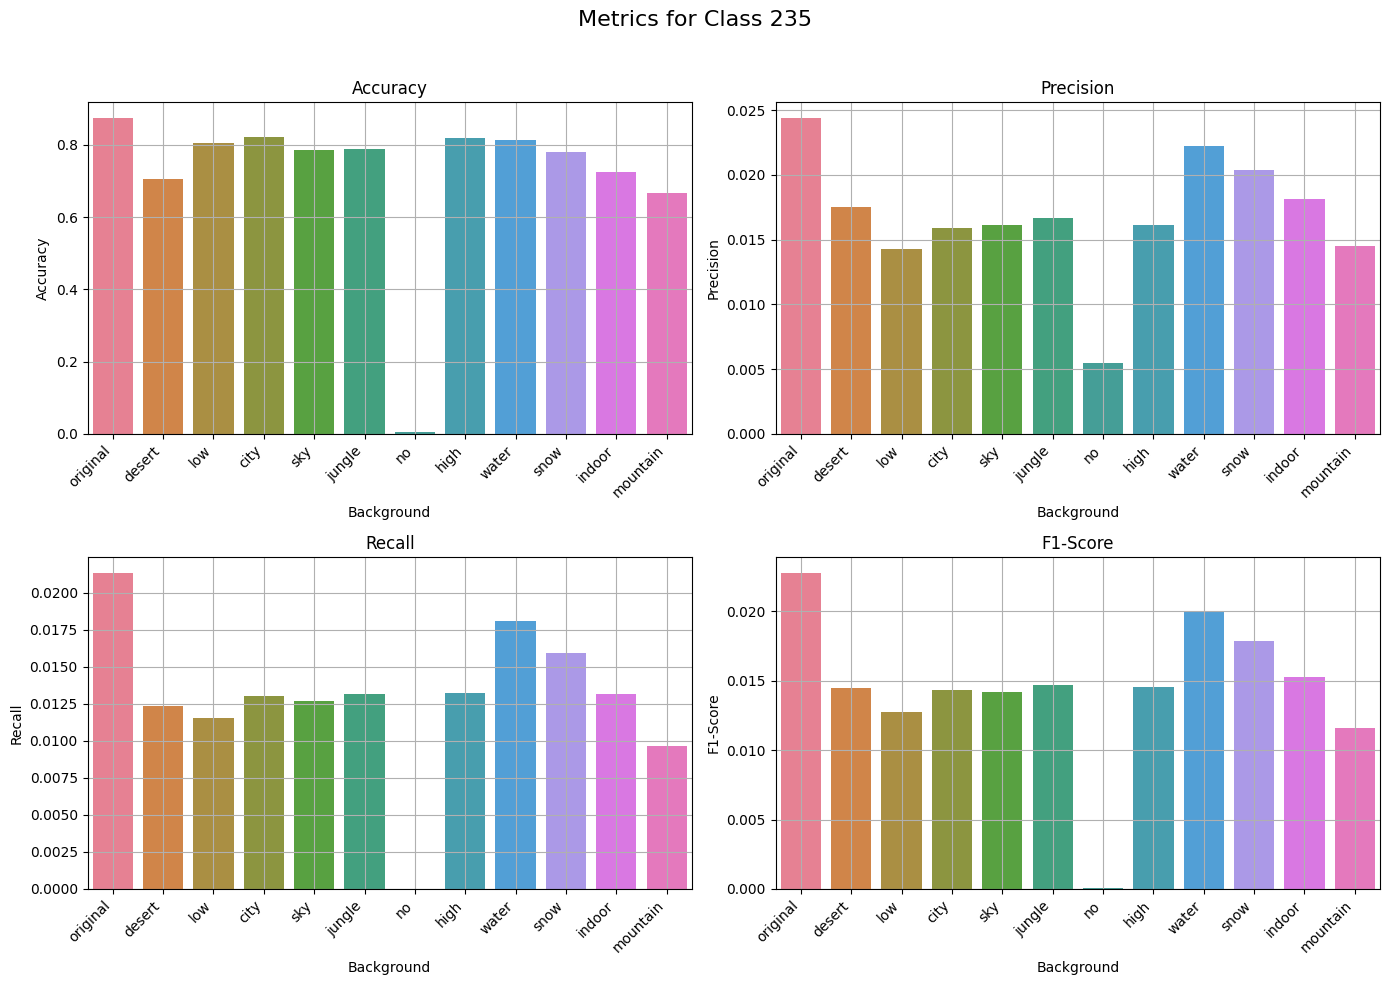
\includegraphics[width=.9\textwidth]{img/235}
	\caption{Metryki}
	\label{rys:235}
\end{figure}

\begin{figure}
	\centering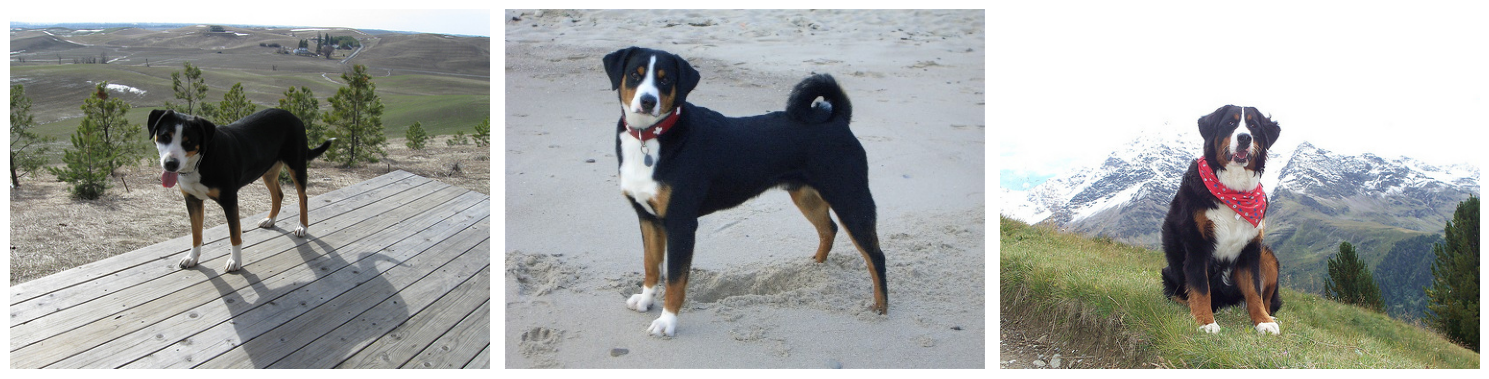
\includegraphics[width=.9\textwidth]{img/238}
	\caption{Metryki}
	\label{rys:238}
\end{figure}

\begin{figure}
	\centering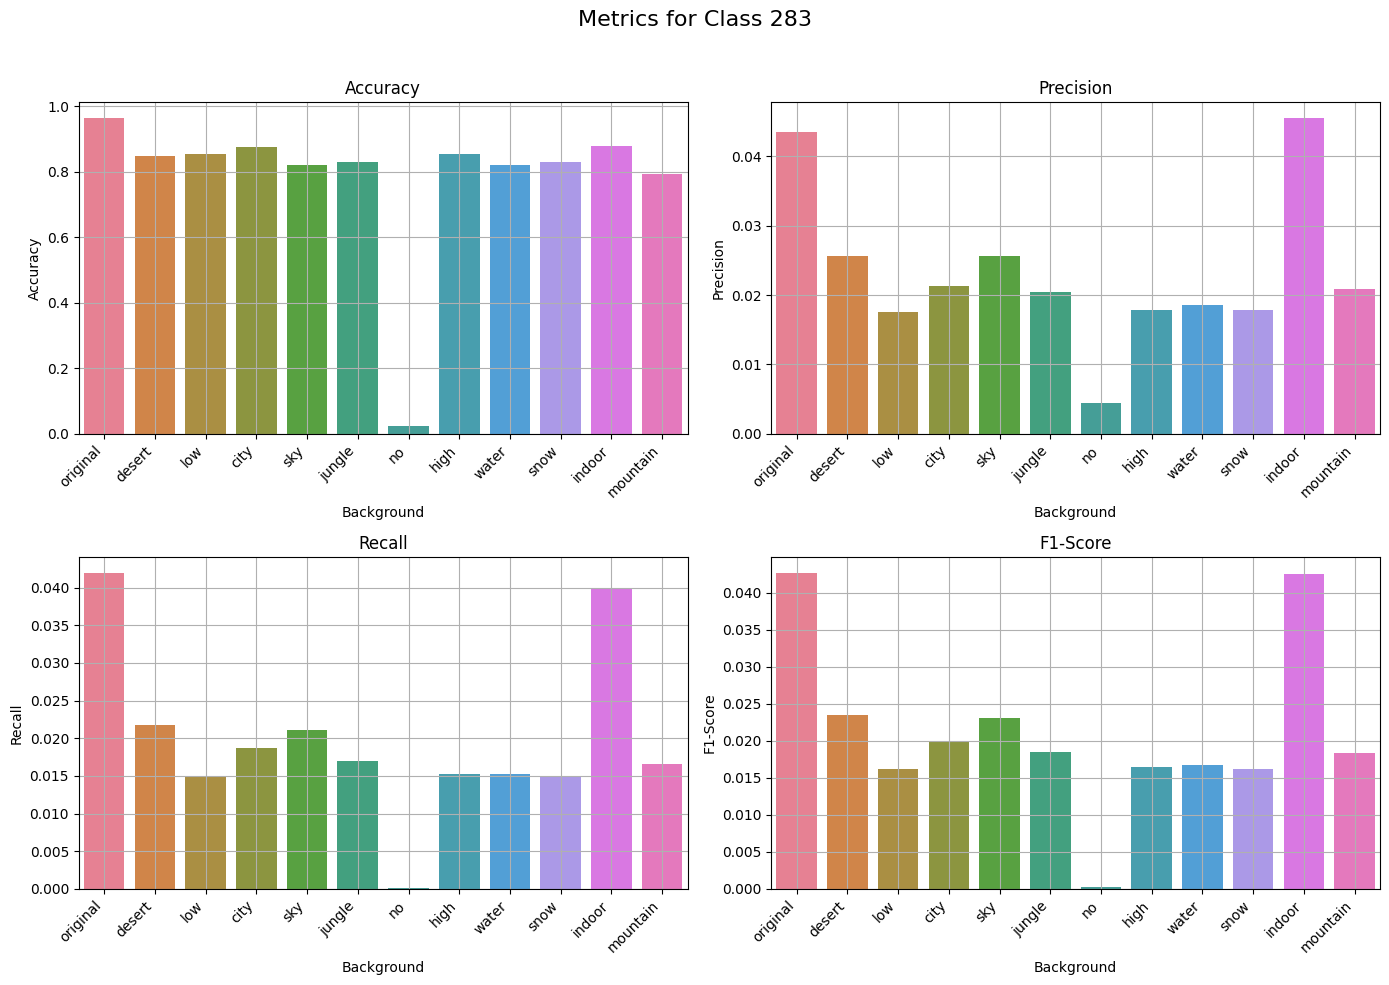
\includegraphics[width=.9\textwidth]{img/283}
	\caption{Metryki}
	\label{rys:283}
\end{figure}

\begin{figure}
	\centering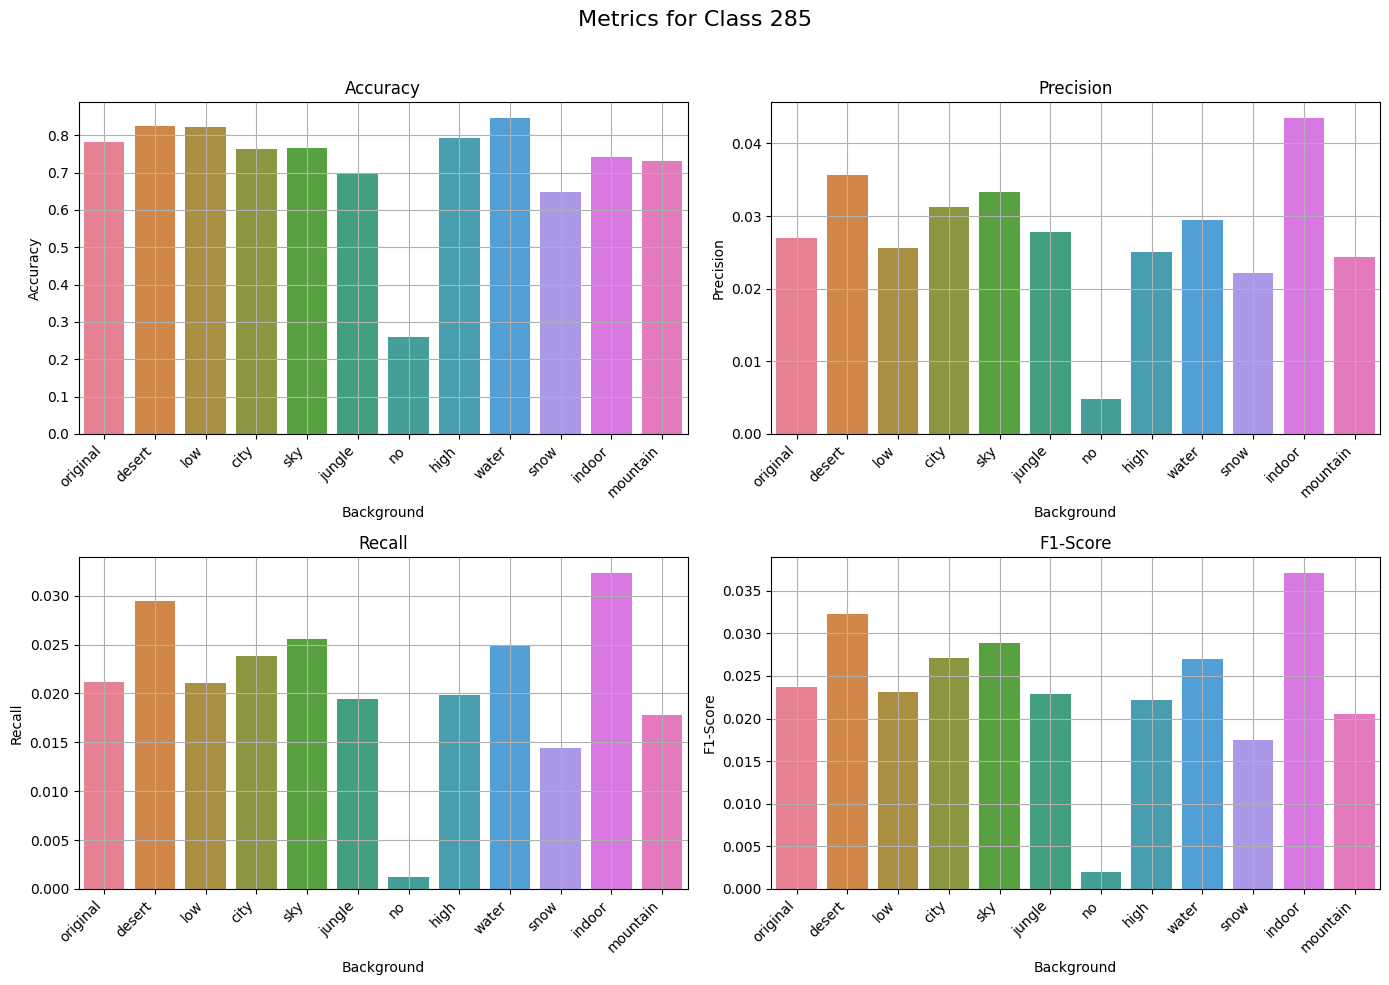
\includegraphics[width=.9\textwidth]{img/285}
	\caption{Metryki}
	\label{rys:285}
\end{figure}

\begin{figure}
	\centering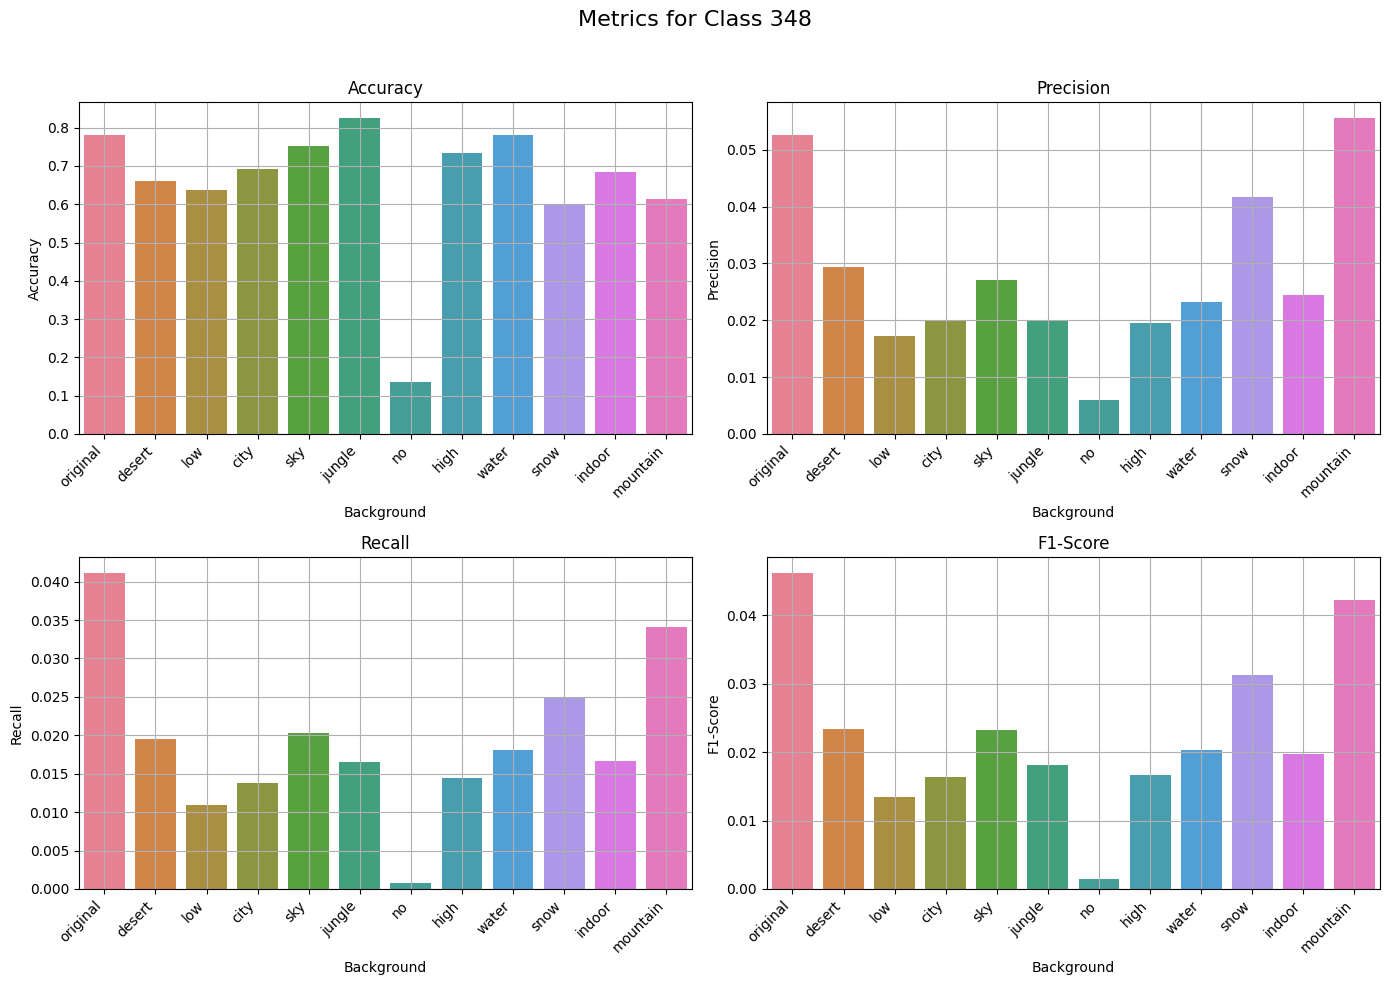
\includegraphics[width=.9\textwidth]{img/348}
	\caption{Metryki}
	\label{rys:348}
\end{figure}

\begin{figure}
	\centering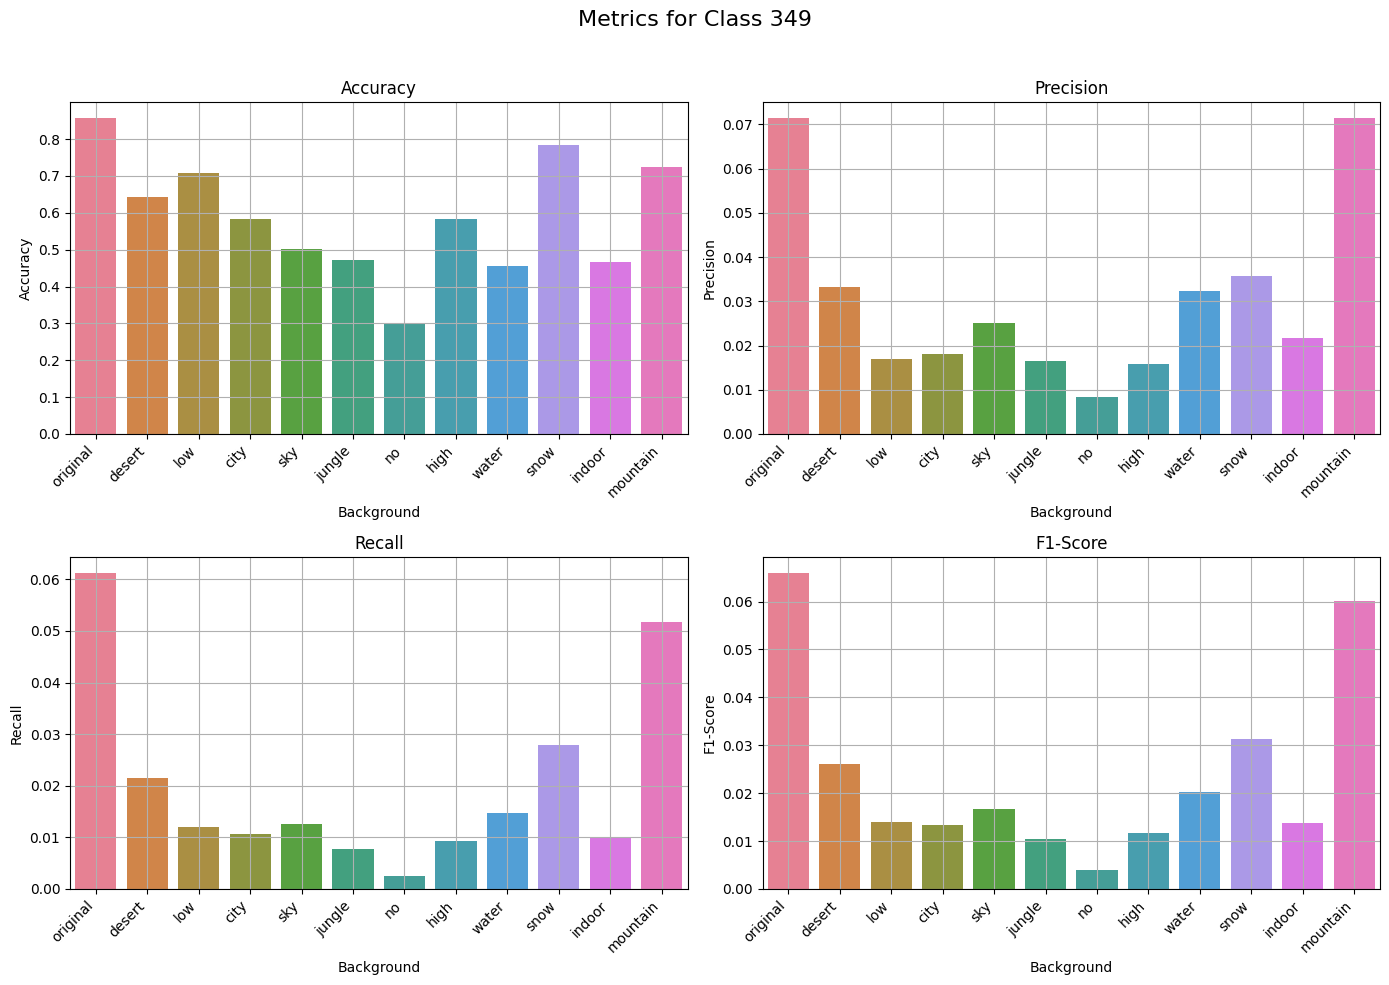
\includegraphics[width=.9\textwidth]{img/349}
	\caption{Metryki}
	\label{rys:349}
\end{figure}


% !TEX encoding = UTF-8 Unicode 
% !TEX root = praca.tex

\chapter*{Podsumowanie}

Analiza wyników klasyfikacji dwóch modeli – ResNet oraz ConvNeXt – wykazała, że modyfikacje tła mają znaczący wpływ na jakość klasyfikacji w obu modelach. Stwierdzono, że wielkość tego wpływu jest zależna od konkretnego modelu, klasy 
zwierzęcia, proporcji obiektu do całego zdjęcia oraz metody modyfikacji tła. Modele często popełniały błędy w przypadku zdjęć z różnorodnym tłem, co sugeruje, że w dużym stopniu polegają na informacjach zawartych w tle podczas procesu 
klasyfikacji.

Model ConvNeXt, reprezentujący nowszą architekturę, uzyskał lepsze wyniki metryk zarówno dla oryginalnych, jak i zmodyfikowanych zdjęć, jednak charakteryzował się mniejszą pewnością swoich decyzji w porównaniu do modelu ResNet. Wyizolowanie 
obiektu poprzez pozostawienie jednolitego koloru tła w niektórych przypadkach poprawiało dokładność, jednak w większości przypadków nieznacznie obniżało wartości metryk. Sugeruje to, że tło może dostarczać modeli cennych informacji, które 
pomagają w poprawnej klasyfikacji, jednak czasami wprowadza także zakłócenia, które mogą mylić model.

Wyniki badania podkreślają znaczenie zróżnicowanych scenerii, obejmujących różne skale, tła i oświetlenie, w procesie uczenia modeli klasyfikacyjnych. Taka różnorodność pomaga zabezpieczyć model przed sytuacjami, w których zdjęcia są wykonane 
w nietypowej scenerii, co może prowadzić do błędnej klasyfikacji. Konkludując, zrozumienie wpływu tła na klasyfikację obrazów jest kluczowe dla poprawy wydajności modeli uczenia maszynowego i może przyczynić się do opracowania bardziej 
odpornych na zakłócenia systemów klasyfikacyjnych.



% Bibliography
\bibliographystyle{dyplom}
\bibliography{bibliography}

% Lists of figures, listings, tables
\listoffigures
\listoflistings
\listoftables

% Appendices - comment out if not applicable
\appendixpage
\appendix
\input{}

\end{document}
